\section{Método propuesto}
\subsection*{}
\begin{frame}{Detección de objetos} % o puntos característicos y descriptores?
  \begin{itemize}
  \item Buscar en una imagen o un video (secuencia de imágenes) un objeto particular dado.
      \note[item]{El reconocimiento de objetos se puede resumir en el objetivo de }
      \note[item]{de forma que estos permitan distinguirla de otras sin la necesidad de tener que analizar la totalidad de la imagen.}
  \item Seleccionar algunos puntos como características distintivas del objeto en la imagen.
    \note[item]{Marcelo: Una de las formas de hacer esto es mediante la detección de puntos claves....* OJO EXISTEN OTRAS FORMAS DE DETECTAR LOS OBJETOS NO SOLO MEDIANTE PUNTUALES... UNA FORMA....}
    \note[item]{(una cantidad suficiente) que sean distinguibles, estables, posean repetibilidad y puedan localizarse.}
    \note[item]{Cuando se tienen imágenes de una misma escena, las correspondencias 2D pueden ser extraídas en cada fotograma para estimar la posición del objeto buscado mediante la identificación de puntos característicos naturales,}
    \note[item]{Una característica local puede ser interpretada como un patrón de imagen que difiere de su vecindad}
    \note[item]{puede venir representada por ejemplo por un punto, un borde o pequeños trozos de la imagen}
  \item La búsqueda de estos puntos, se puede realizar mediante detectores de puntos claves.
  \item Se representa la vecindad de cada punto de interés detectado mediante un vector descriptor.
      \note[item]{Es común la realización de ciertos cálculos sobre una región alrededor de la característica local detectada y su resultado se convierte en un vector numérico el cual recibe el nombre de descriptor}
      \note[item]{Idealmente, este descriptor debe ser distintivo, robusto al ruido, a la detección de desplazamientos y a las deformaciones geométricas o fotométricas de la imagen.}
  \item Se buscan las correspondencias entre los vectores descriptores de las imágenes. 
    \note[item]{La dimensión del descriptor impacta directamente en el tiempo de cálculo y distintividad.}
    \note[item] {Estos detectores son la base de gran cantidad de herramientas basadas en visión computacional(reconocimiento de objetos, vigilancia por video, imágenes médicas, la realidad aumentada, etc.)} 

\note[item]{Características locales: Cuando se trabaja con características locales uno de los primeros inconvenientes a resolver es obtener un alto nivel de invarianza: esto depende de las deformaciones geométricas y fotométricas que pueda sufrir la imagen.
 \begin{itemize}
  \item Nos centraremos en: cambios de escala, la rotación en el plano,
  \item Se asume que los efectos de segundo orden: inclinación, perspectiva y anisotropía son cubiertos en cierto grado por la robustez global del descriptor utilizado
  \item En cuanto a las deformaciones fotométricas, se asume un modelo lineal simple con un desplazamiento y un cambio de contraste (factor de escala).
 \end{itemize}
}
% \subsection{Realidad Aumentada}
  \end{itemize}
\end{frame}
\subsection*{Método}
\subsubsection*{Etapas}
\begin{frame}{Etapas}
\note[item]{El método propuesto posee 2 etapas}
  \begin{block}{Configuración}
   \begin{itemize}
    \item Se realiza una sola vez al inicio del algoritmo.
    \item Se registra la imagen que posteriormente se detectará en el flujo de video.
   \end{itemize}
  \end{block}
  \begin{block}{Ejecución}
	\note[item]{Marcelo: 
	  aplique condicionales
	  se resuelven incongruencias en transformaciones
	  aumenta la velocidad de procesamiento
	  resulta sin flickering
	}
   \begin{itemize}
    \item Captura de un frame del flujo de video proporcionado por la cámara web.
    \item Procesamiento para detectar el objeto registrado en la Configuración.
    \item Superposición de un objeto virtual para enriquecer la realidad.
   \end{itemize}
  \end{block}
\end{frame}
%
\begin{frame}{Etapa de configuración}
	\begin{center}
  	  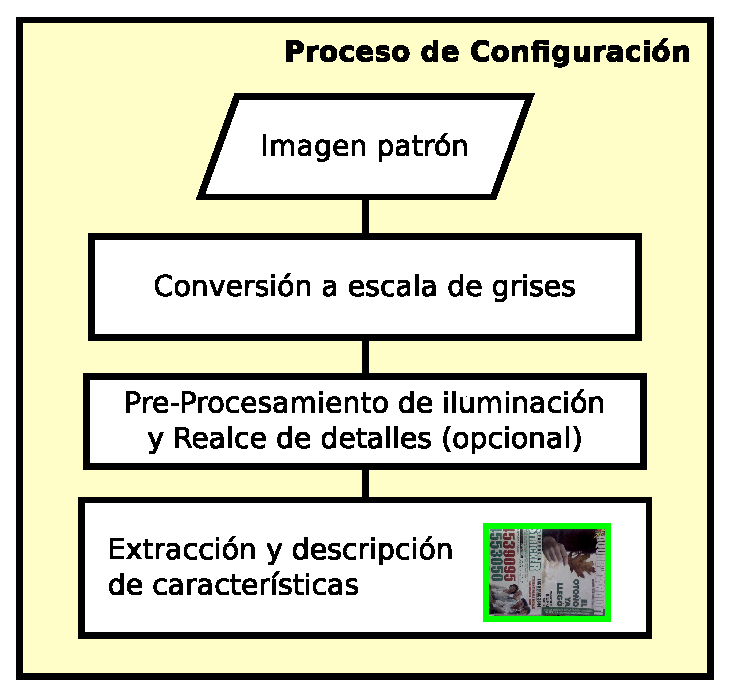
\includegraphics[scale=0.5]{../../figs/proceso_completo_entrenamiento_presentacion}
	\end{center}
\end{frame}
%
\begin{frame}{Etapa de ejecución}
	\note[item]{Marcelo: antes de explicar etapa 2: decir que hace el método estandar. Existe un método.. o algo asi...}
	\begin{center}
  	  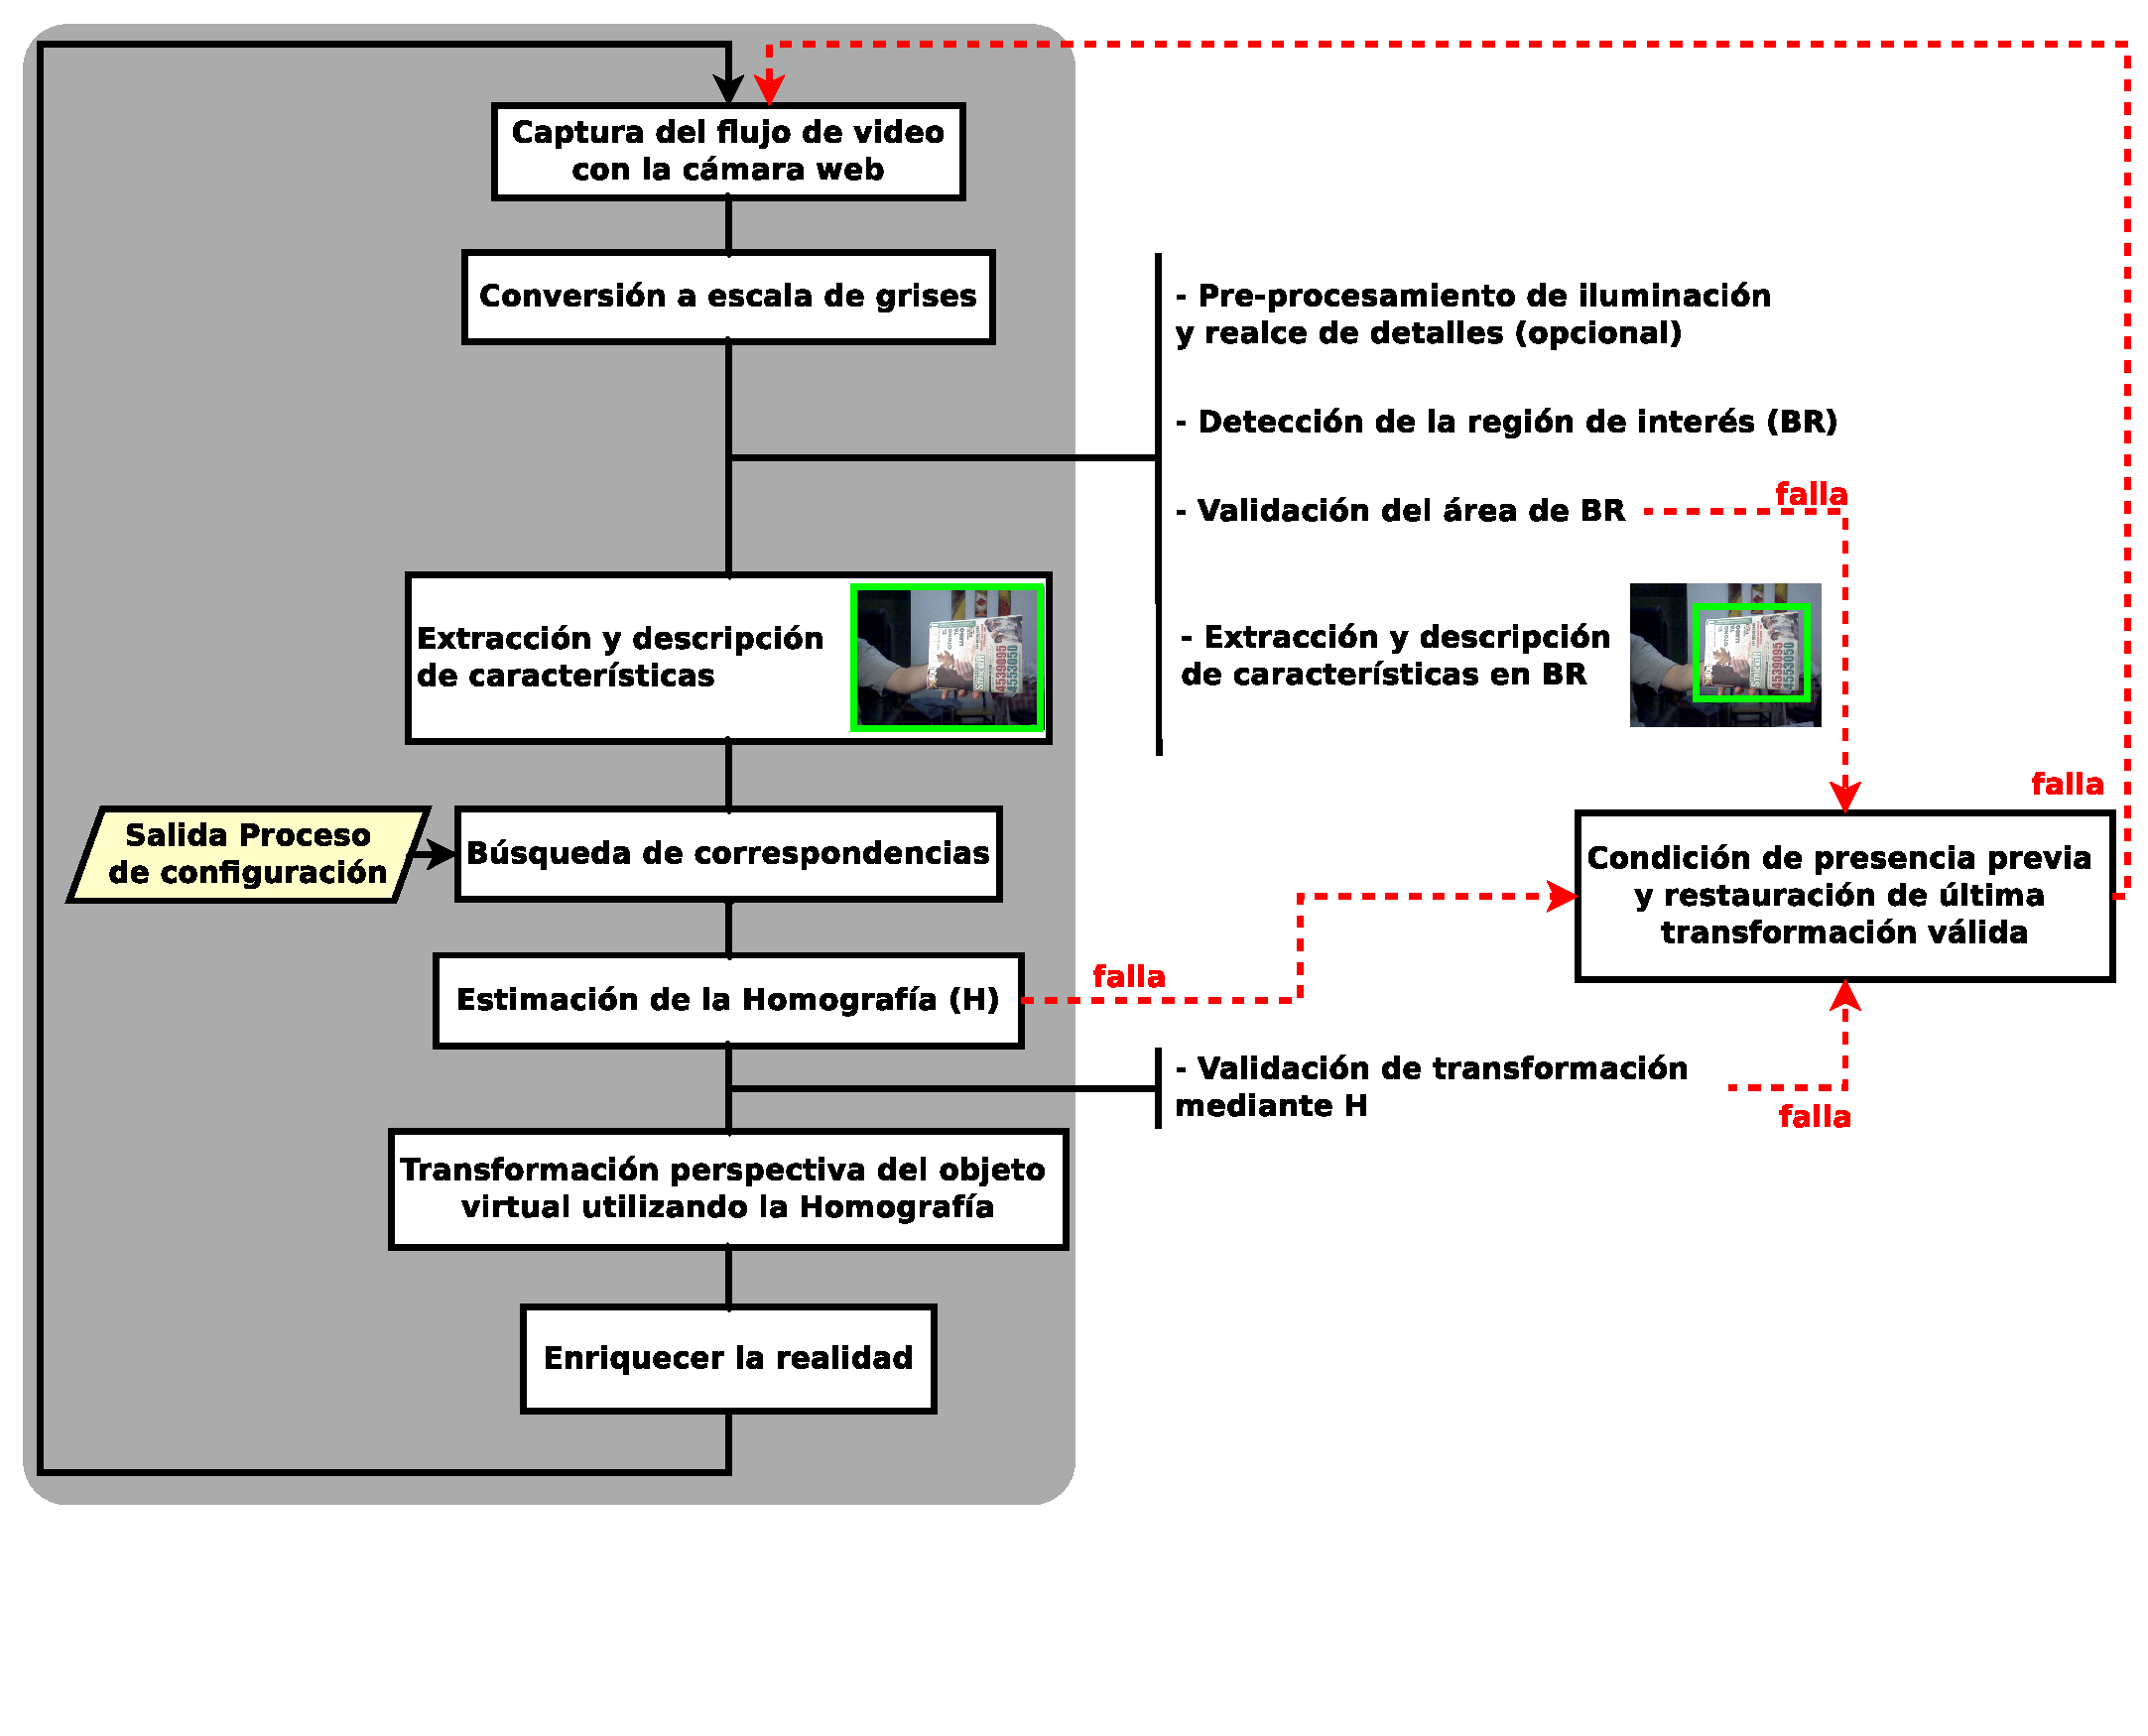
\includegraphics[scale=0.29]{../../figs/proceso_completo_presentacion_negrita} %proceso_completo_presentacion1
	\end{center}
\end{frame}

% \begin{frame}{Etapa de ejecución}
%     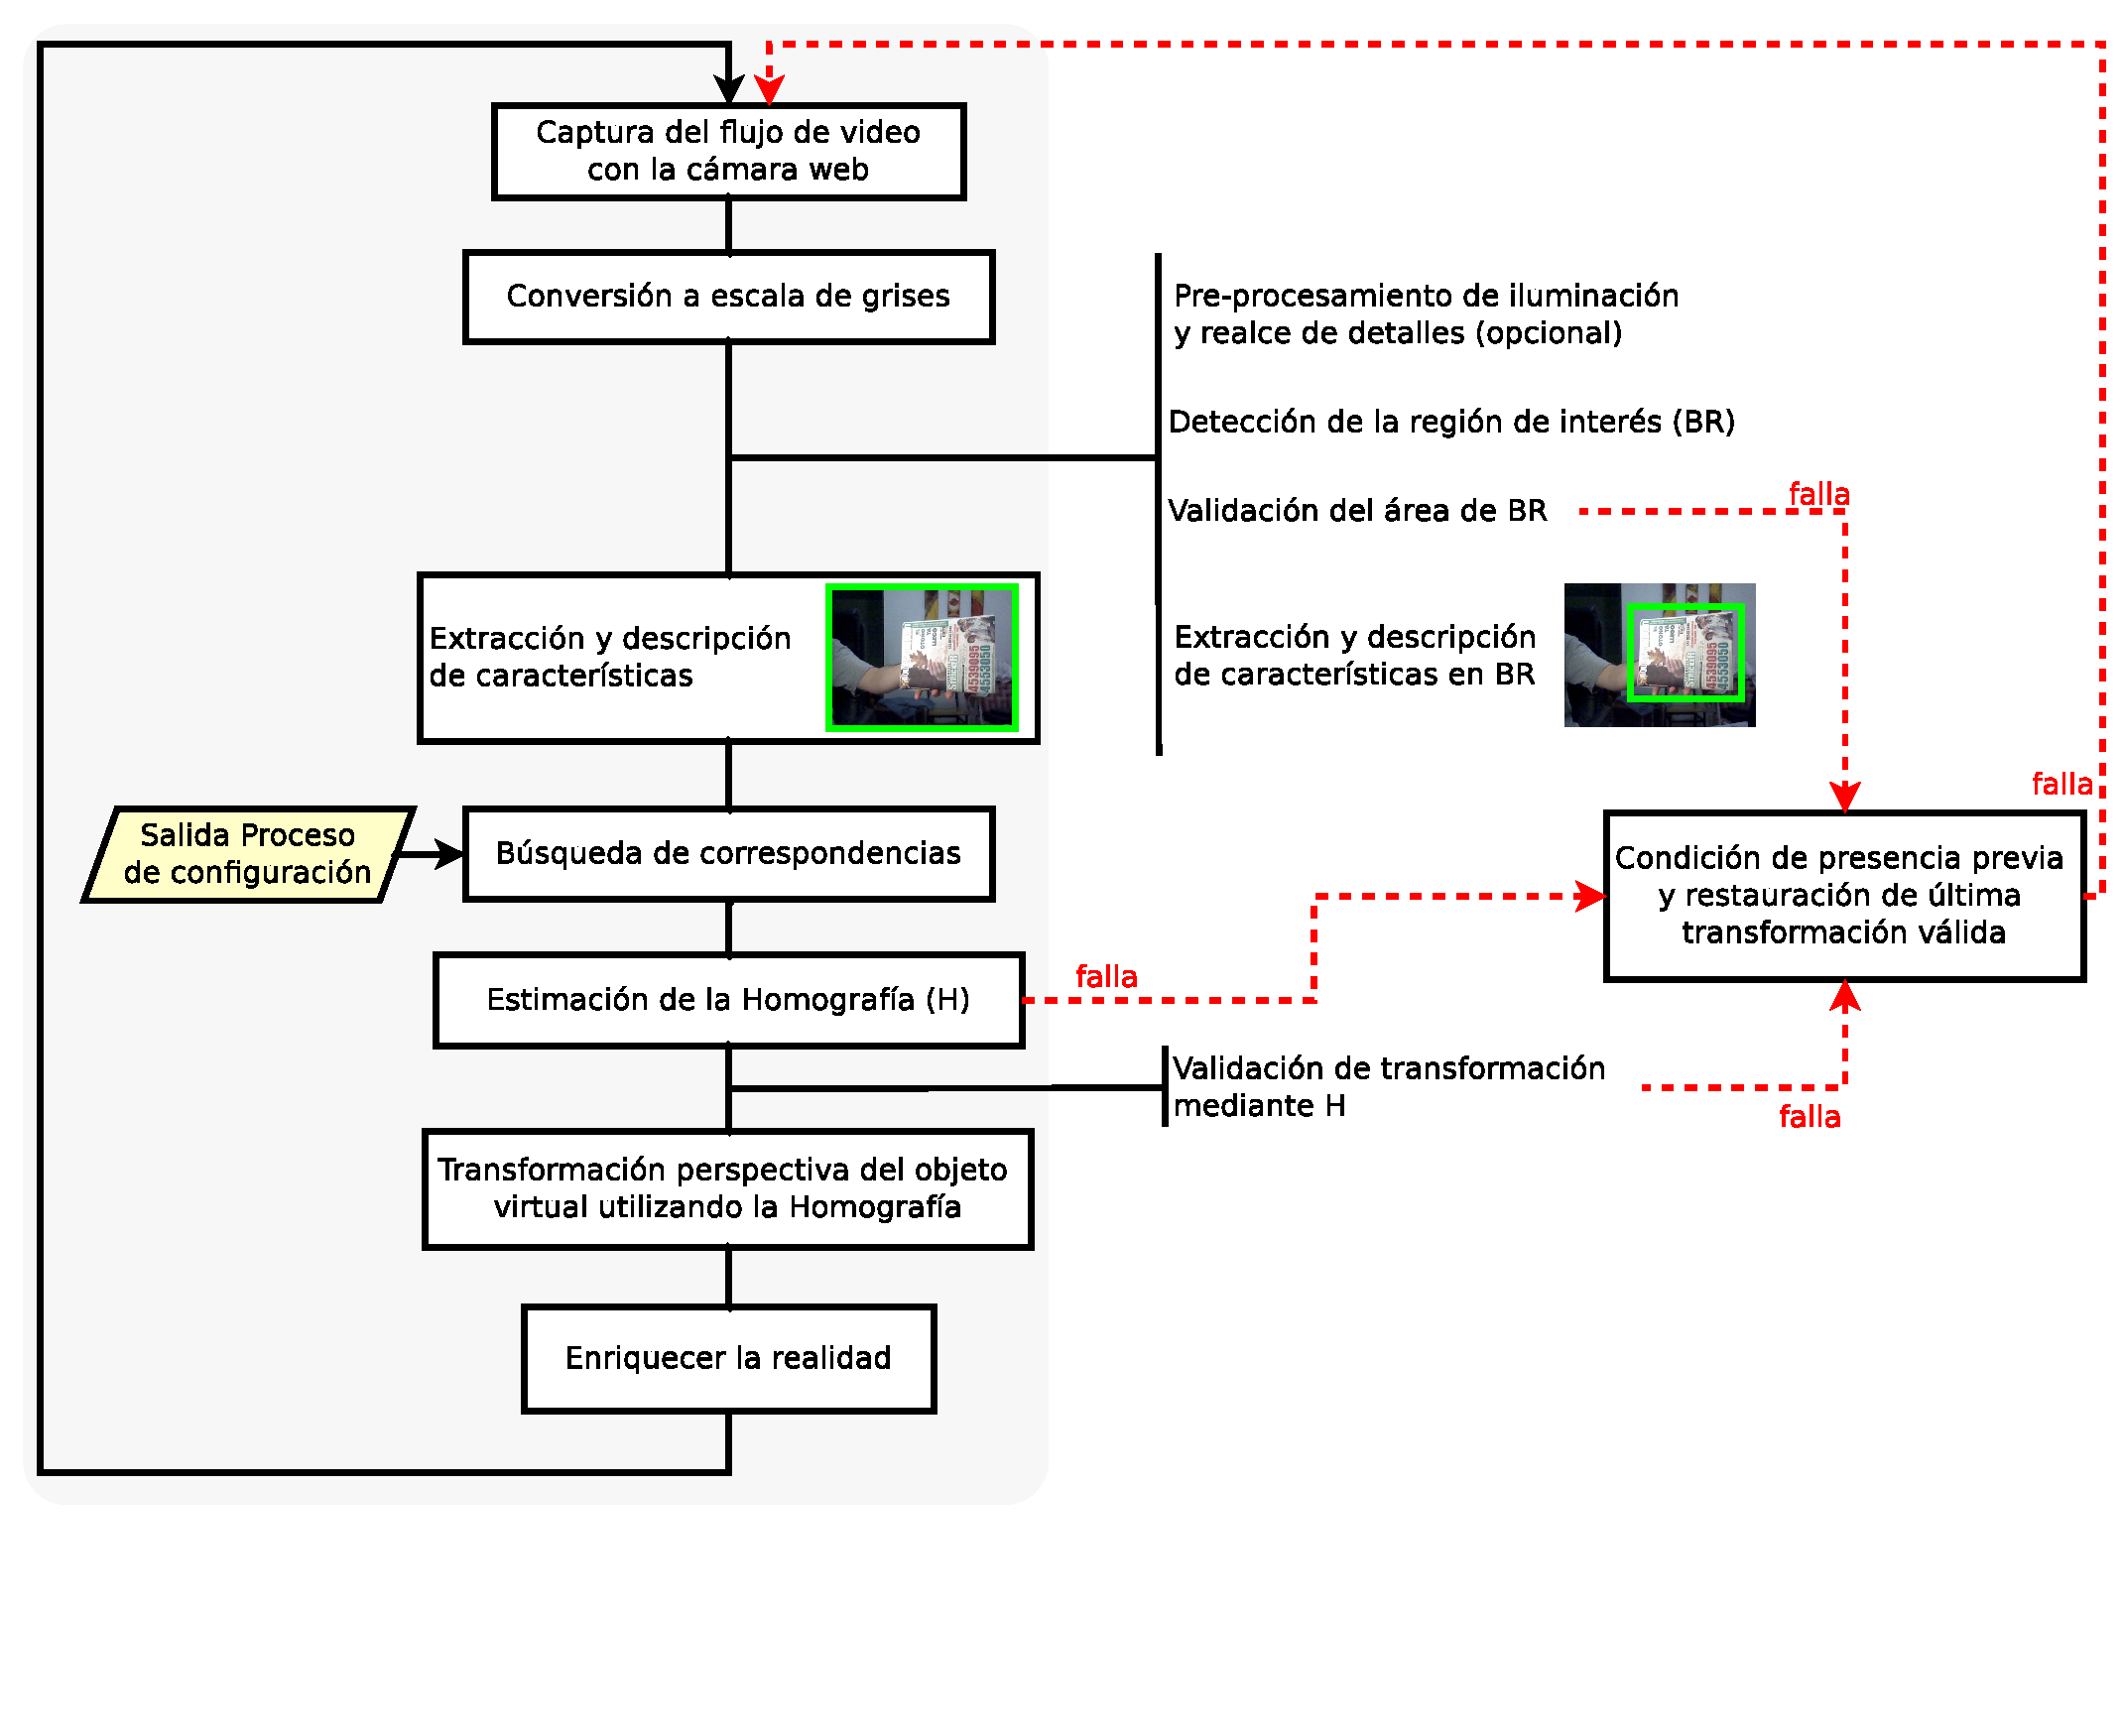
\includegraphics[scale=0.2]{../../figs/proceso_completo_presentacion}
%     \framezoom<1><1>[border](0cm, 0cm)(2.5cm, 3.4cm)
% \end{frame}
% \begin{frame}{Etapa de ejecución}
%     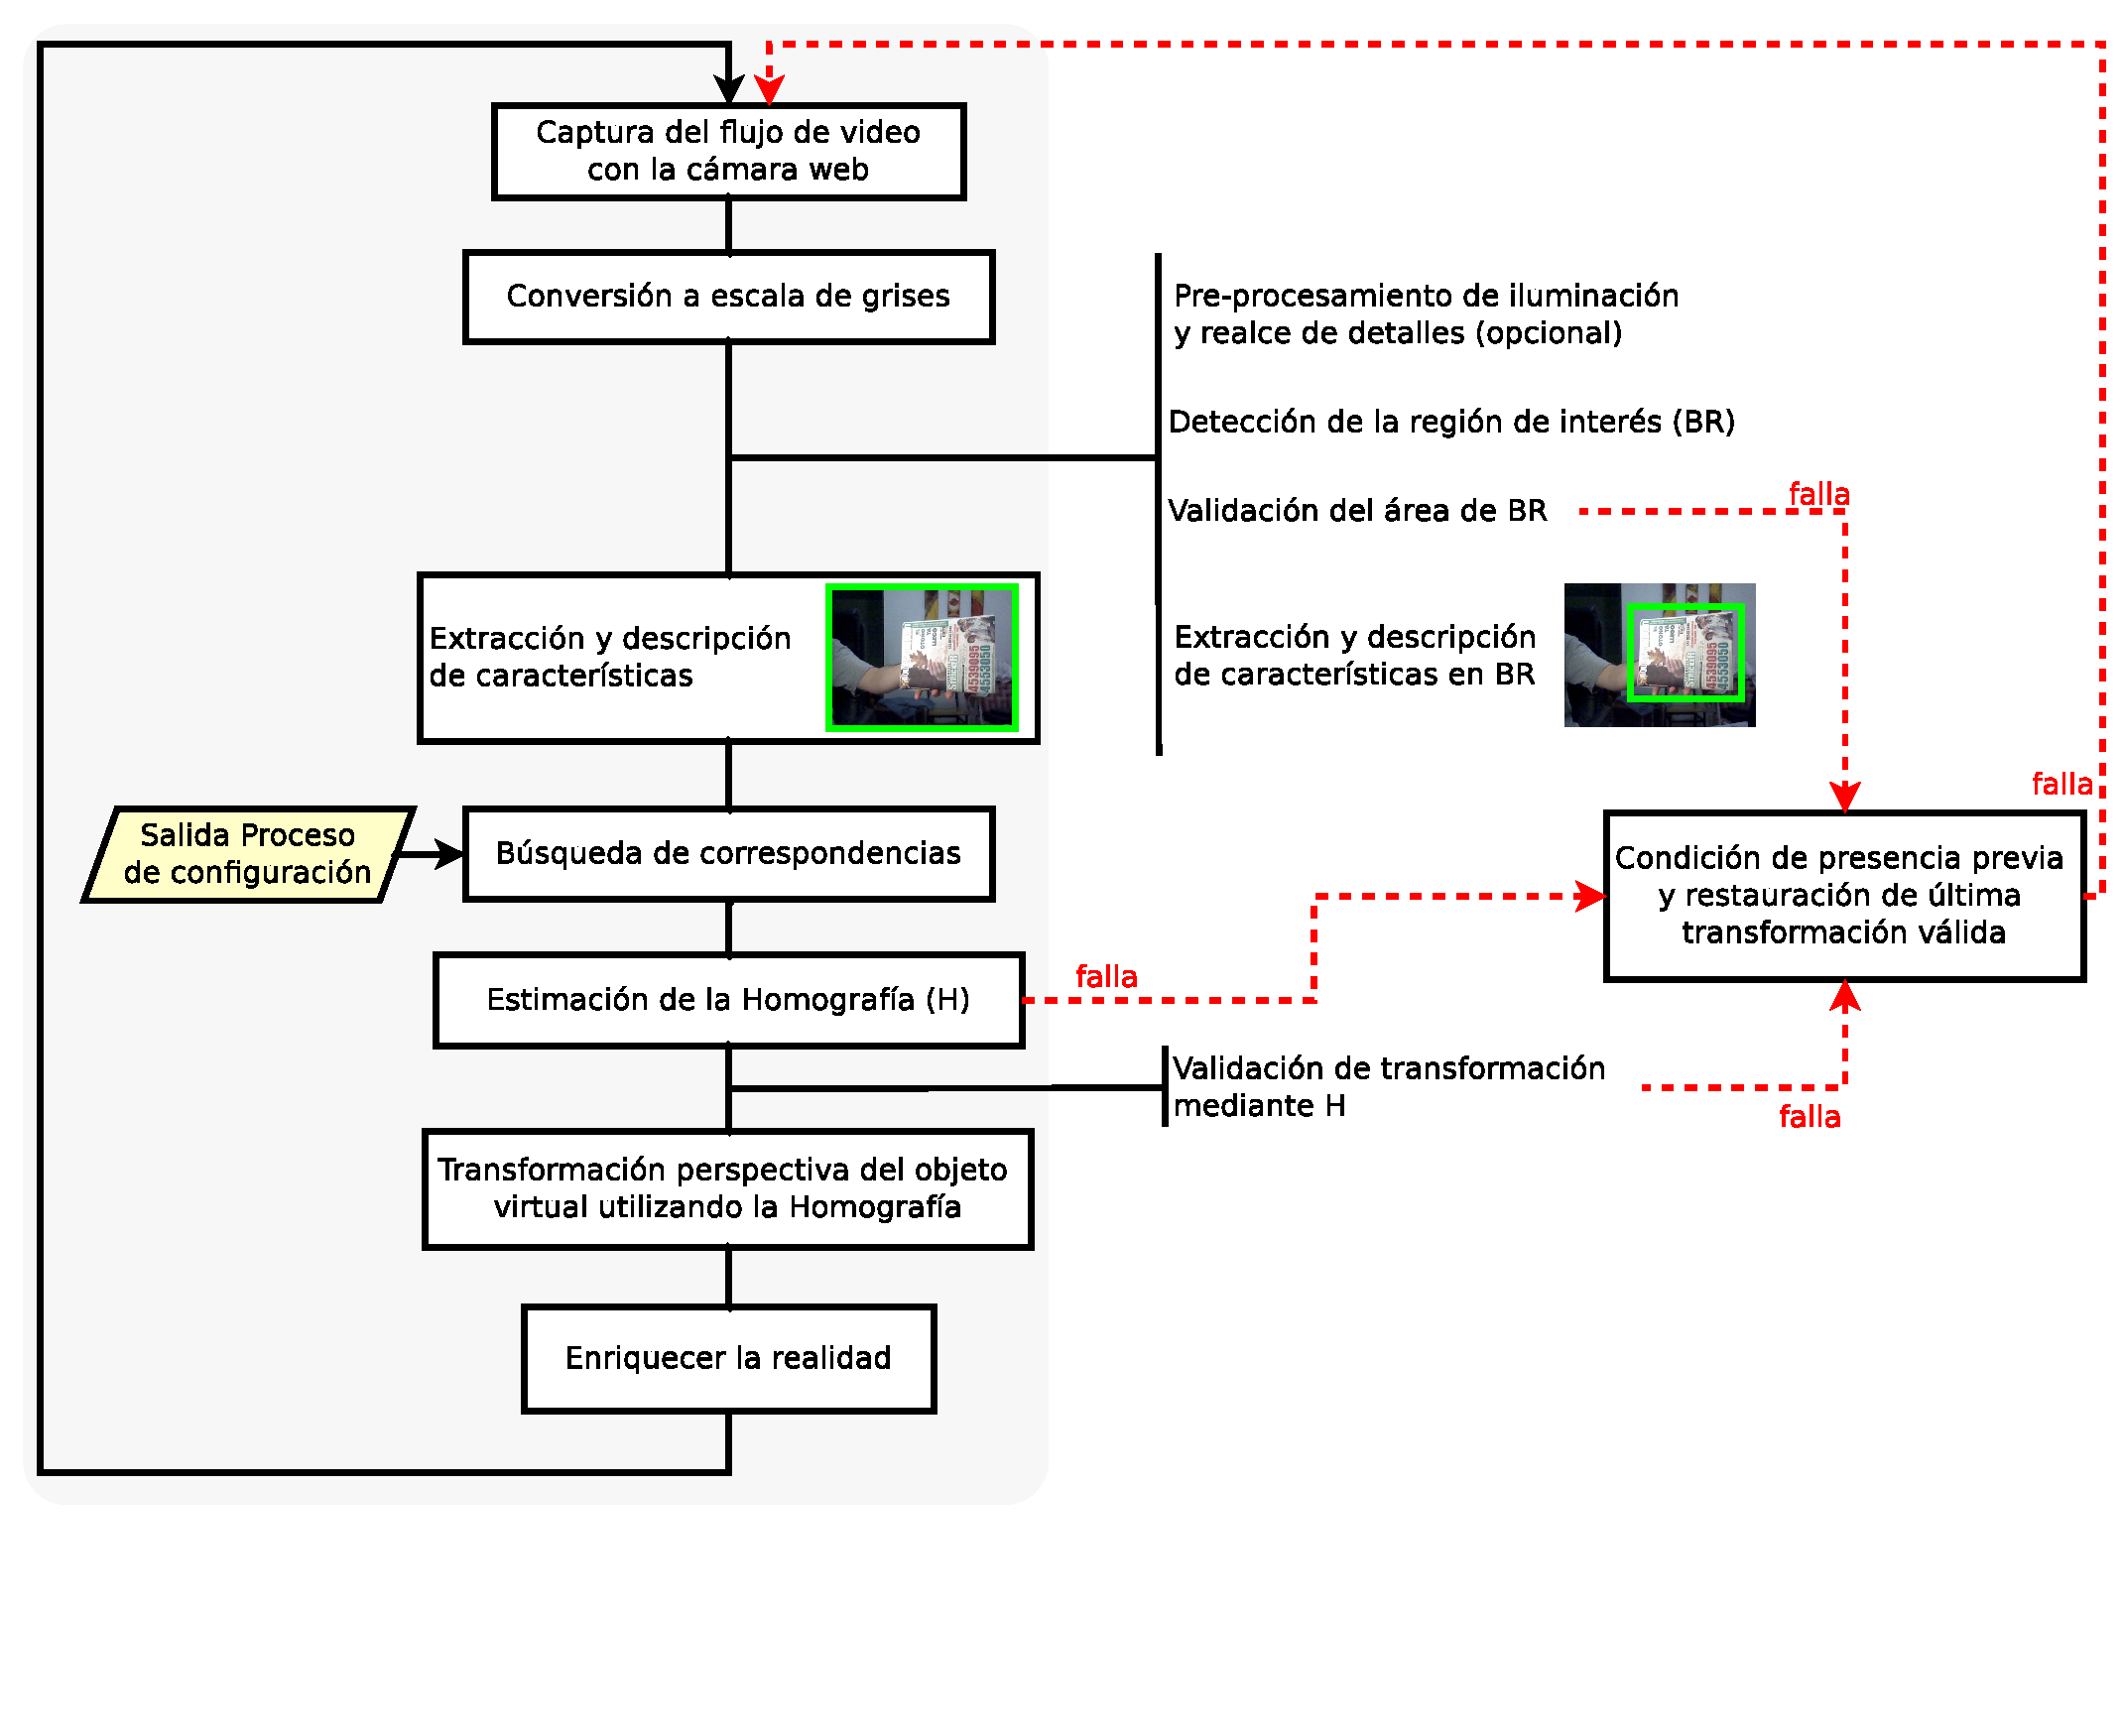
\includegraphics[scale=0.2]{../../figs/proceso_completo_presentacion}
%     \framezoom<2><1>[border](0cm, 3.4cm)(3cm, 3.4cm)
% \end{frame}

\subsection*{}
\begin{frame}{Conversión a escala de grises}
	Formula perceptualmente ponderada:
	\begin{equation*}
	  \label{eq:formula_conv_grises}
	  I=0.299R+0.587G+0.114B.
	\end{equation*}
\end{frame}

\begin{frame}{Pre-procesamiento de realce de detalles y mejora en iluminación}
    \begin{itemize}
      \item Transformación logarítmica 
	$\hspace{0.2cm}
	  s=\;log(1+r) 
	  \label{eq:logaritmo}
	$.
	\note[item]{utilizada cuando la imagen de entrada tiene un rango dinámico grande, expande las intensidades oscuras y comprime las intensidades claras... Los oscuros se ven mas claros y los claros aún mas claros}
      \item Ecualización del histograma.
	\note[item]{Es una función que describe de manera global la apariencia de una imagen. Puede interpretarse como el número de píxeles en función de las intensidades de grises.}
	\note[item]{Pretende obtener el mismo número de píxeles para cada nivel de gris (distribución que se aproxima a la uniforme).}
	\note[item]{Se obtiene una expansión en el rango dinámico de la imagen - aumento del contraste.}
      \item Filtrado pasa altos: \note[item]{realza las altas frecuencias - realza los detalles}
	\note[item]{puede ser aplicado mediante la convolución de la imagen con un kernel pasa altos. Si la suma de los coeficientes del kernel es 1, se realzan las altas frecuencias conservándose el brillo medio de la imagen sobre la cual se aplica el filtro.}
	\small{
	\begin{equation*}
	  g(x,y)=\sum_{s=-a}^{a}\sum_{\; t=-b}^{a}w(s,t)f(x+s,y+t)\label{eq:ec_convolucion}
	  \hspace{0.2cm}
	  w=\begin{bmatrix}
	  \quad0 & -1 & \quad0\\
	  -1 & \quad5 & -1\\
	  \quad0 & -1 & \quad0
	  \end{bmatrix}
	\end{equation*}}
	 \item Filtrado de alta potencia: 
	      \note[item]{se obtiene entre una versión amplificada de la imagen original y una versión suavizada de la misma}
	      \small{\begin{equation*}
		\label{eq:form_alta_potencia}
		g(x,y)=(A-1)f(x,y)+PA(f(x,y)) \hspace{0.2cm} \textrm{con} \hspace{0.2cm} A=2;
		\hspace{0.2cm} kernel=\begin{bmatrix}
		-1 & -1 & -1\\
		-1 & \quad8 & -1\\
		-1 & -1 & -1
		\end{bmatrix}
	      \end{equation*}
	    }
	    \note[item]{Formula equivalente: Af\-PB(f)}
      \item Ecualización del histograma y posteriormente filtrado de alta potencia.
	  \note[item]{Realzar el contraste y luego mejora los detalles}
    \end{itemize}
  \end{frame}
  
\subsection{Detección de movimiento}
\begin{frame}{Detección de la región de interés}
  Determinación de una zona de interés para realizar la extracción de características. 
    \note[item]{La región de interés es la parte cambiante del flujo de video}
	\begin{itemize}
		\item Diferencia de imágenes ($F$: cuadro del flujo de video).
		\begin{equation*}
		  D(x,y)=|F_{t}(x,y)-F_{t-1}(x,y)|\;\forall\; x,y\;\in F.
		  \label{eq:diferencia_absoluta}
		\end{equation*} \note[item]{La diferencia no es exacta, y aparece ruido y patrones speckle en la imagen}
		\item Umbral Binario.
		  \note[item]{Marcelo: no explicar umbral de binarización}
		  \note[item]{r y s son variables que denotan el nivel de gris.}
% 		$s=T(r)$
% 		\begin{equation*}
% 		  \label{eq:equation_umbral_binario}
% 		  s= 
% 		  \begin{cases} 0 & \text{para $r<50$,}
% 		  \\
% 		  255 &\text{para $r>=50$}
% 		  \end{cases} \textrm{con } 0 \leq r \leq 255% \textrm{ y } 0 \leq u \leq r_{max}.
% 		\end{equation*}
		\item Erosión $\times$ 2 $\rightarrow$ eliminar puntos aislados. \note[item]{eliminar detalles irrelevantes de una imagen binaria. El tamaño de los objetos se ve reducido y el ruido o detalles irrelevantes es eliminado.}
		\item Dilatación $\times$ 2 $\rightarrow$ recuperar eliminación de objetos de interés. \note[item]{los objetos crecen en su tamaño y algunos de los espacios dentro de ellos son rellenados}
		\item Rectángulo delimitador mínimo (BR).
		    \note[item]{$\rightarrow$ rectángulo más pequeño que encierra todos los puntos con valor diferente de 0.}
		\item Umbral sobre el área de BR
	\end{itemize}
\end{frame}

% \begin{frame}{Erosión y dilatación}
% 	\begin{itemize}
% 		\item Erosión $\rightarrow$ En una imagen erosionada, el tamaño de los objetos se ve reducido y el ruido o detalles irrelevantes (aislados) es eliminado
% 		\item Dilatación $\rightarrow$ los objetos crecen en su tamaño y algunos de los ``espacios'' dentro de ellos son rellenados (complementaria a la Erosión)
% 	\end{itemize}
% 		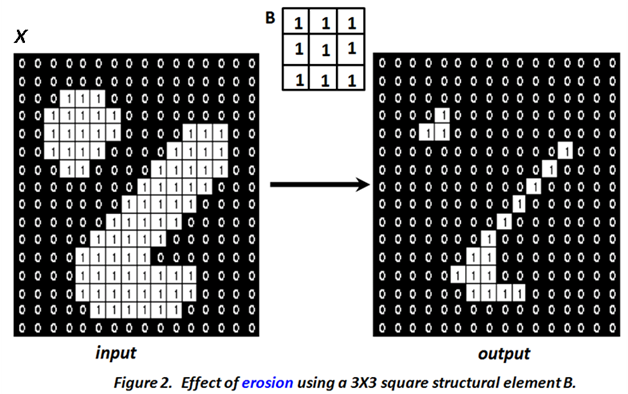
\includegraphics[width=5cm]{./img1/erosion}\qquad
% 		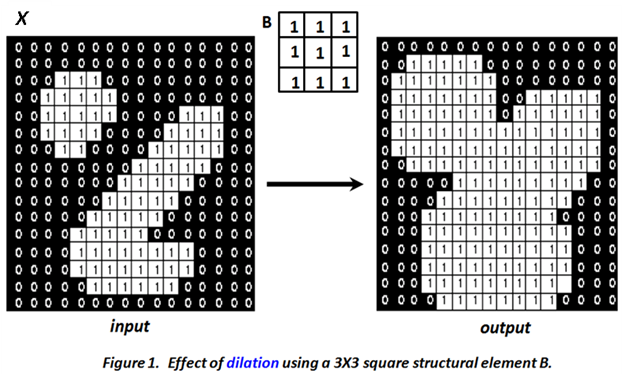
\includegraphics[width=5cm]{./img1/dilation}
% \end{frame}

\begin{frame}{Detección de la región de interés}
  \begin{figure}[tbhp]
    \centering
    \subfloat[][\small{Frame Previo}]{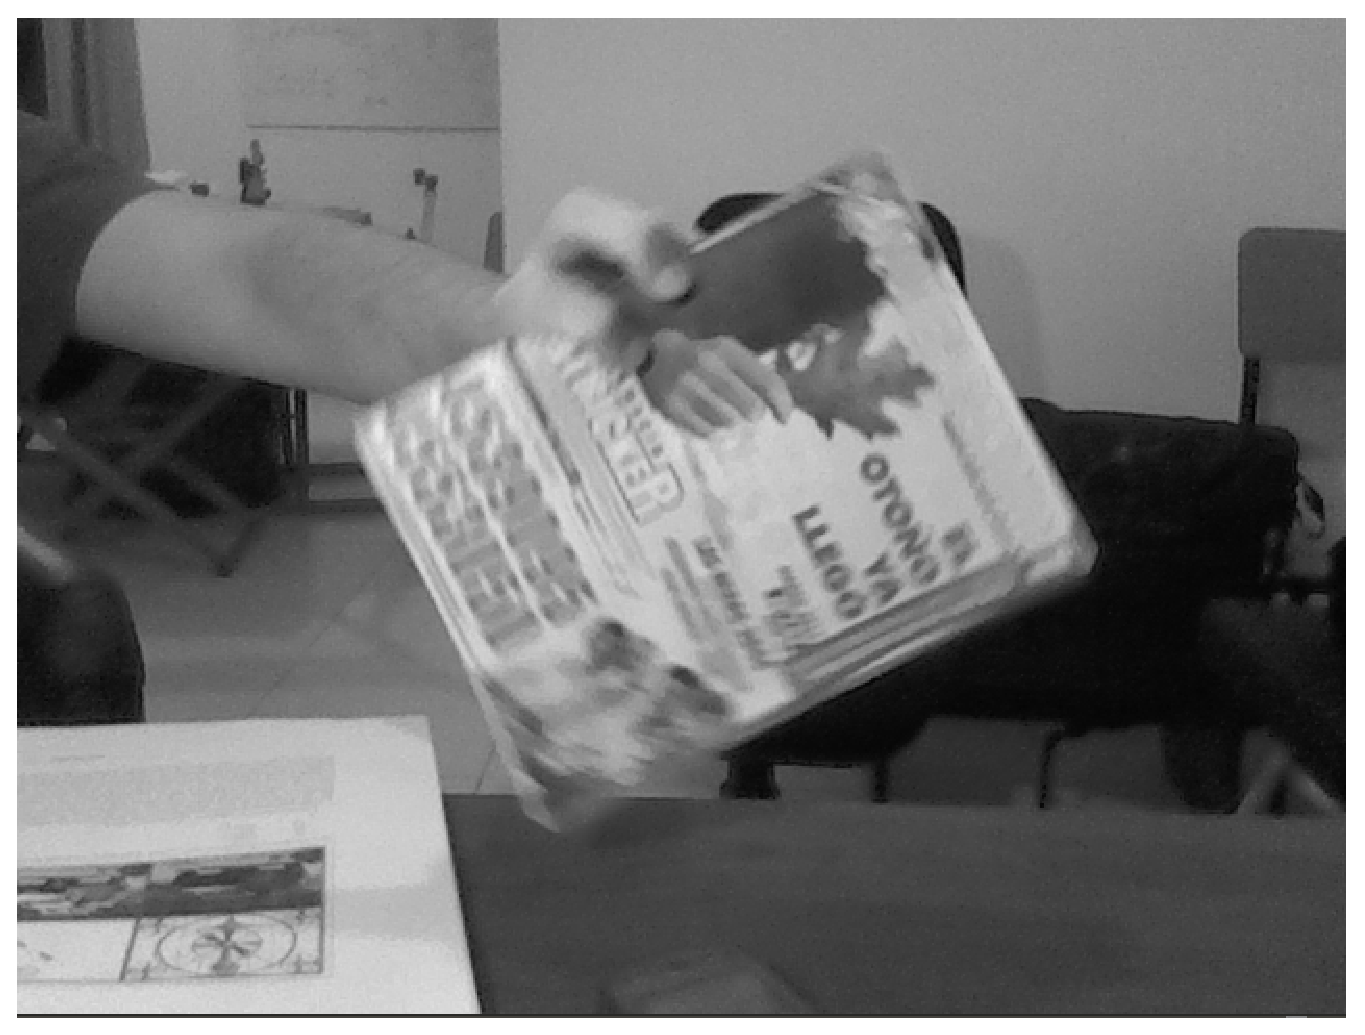
\includegraphics[width=0.27\textwidth]{../../figs/preprocess/srcPrev} \label{fig:deteccion_movimietno-srcprev}}
    \subfloat[][\small{Frame Actual}]{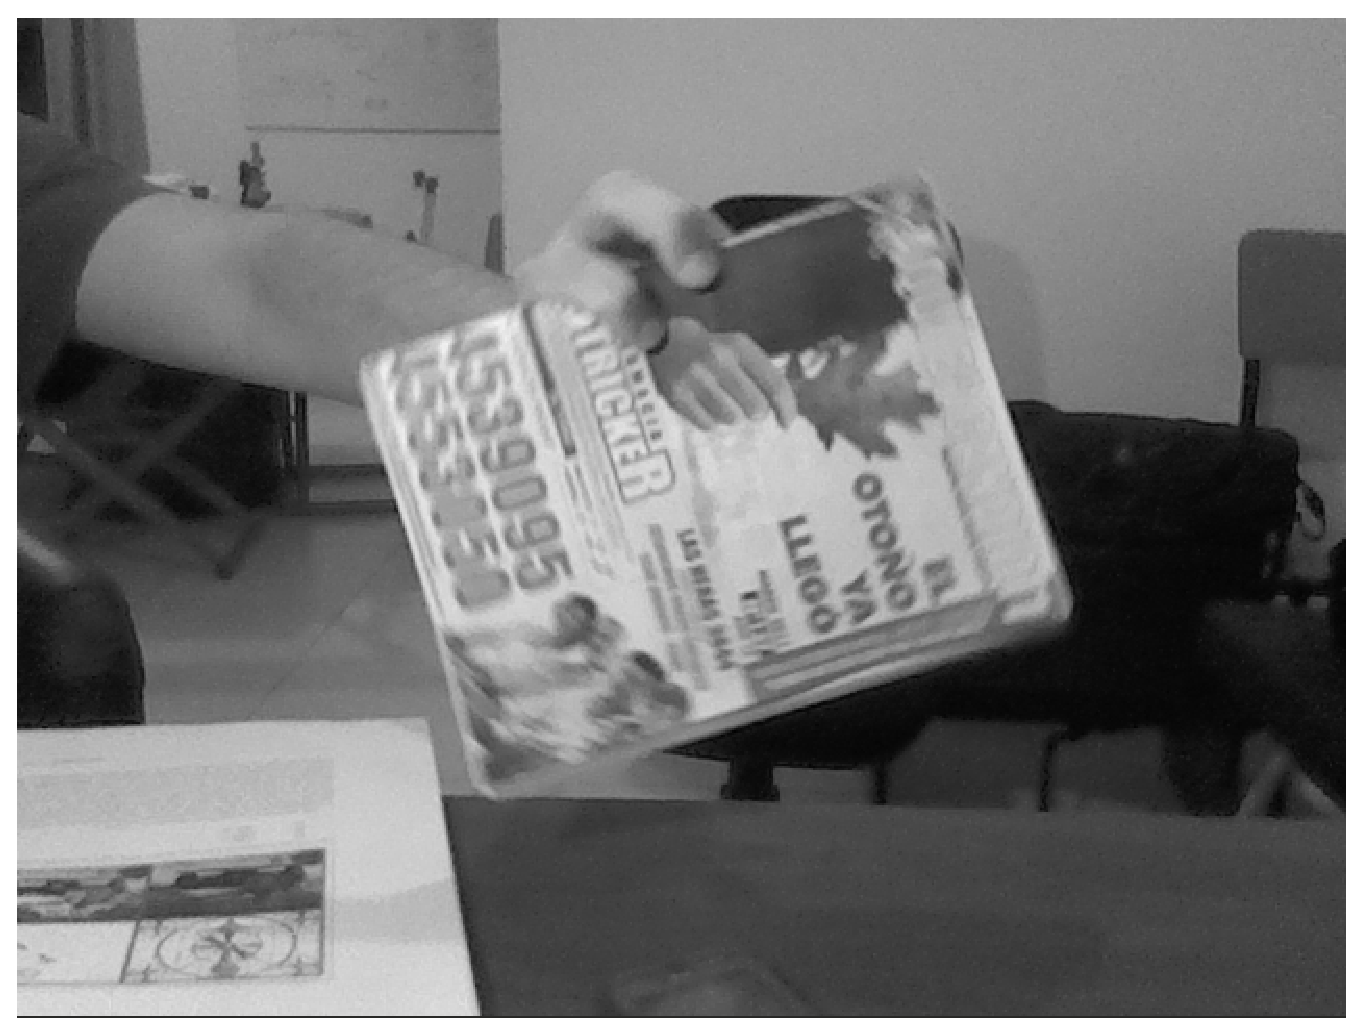
\includegraphics[width=0.27\textwidth]{../../figs/preprocess/src} \label{fig:deteccion_movimietno-src}}
    \subfloat[][\small{Diferencia absoluta}]{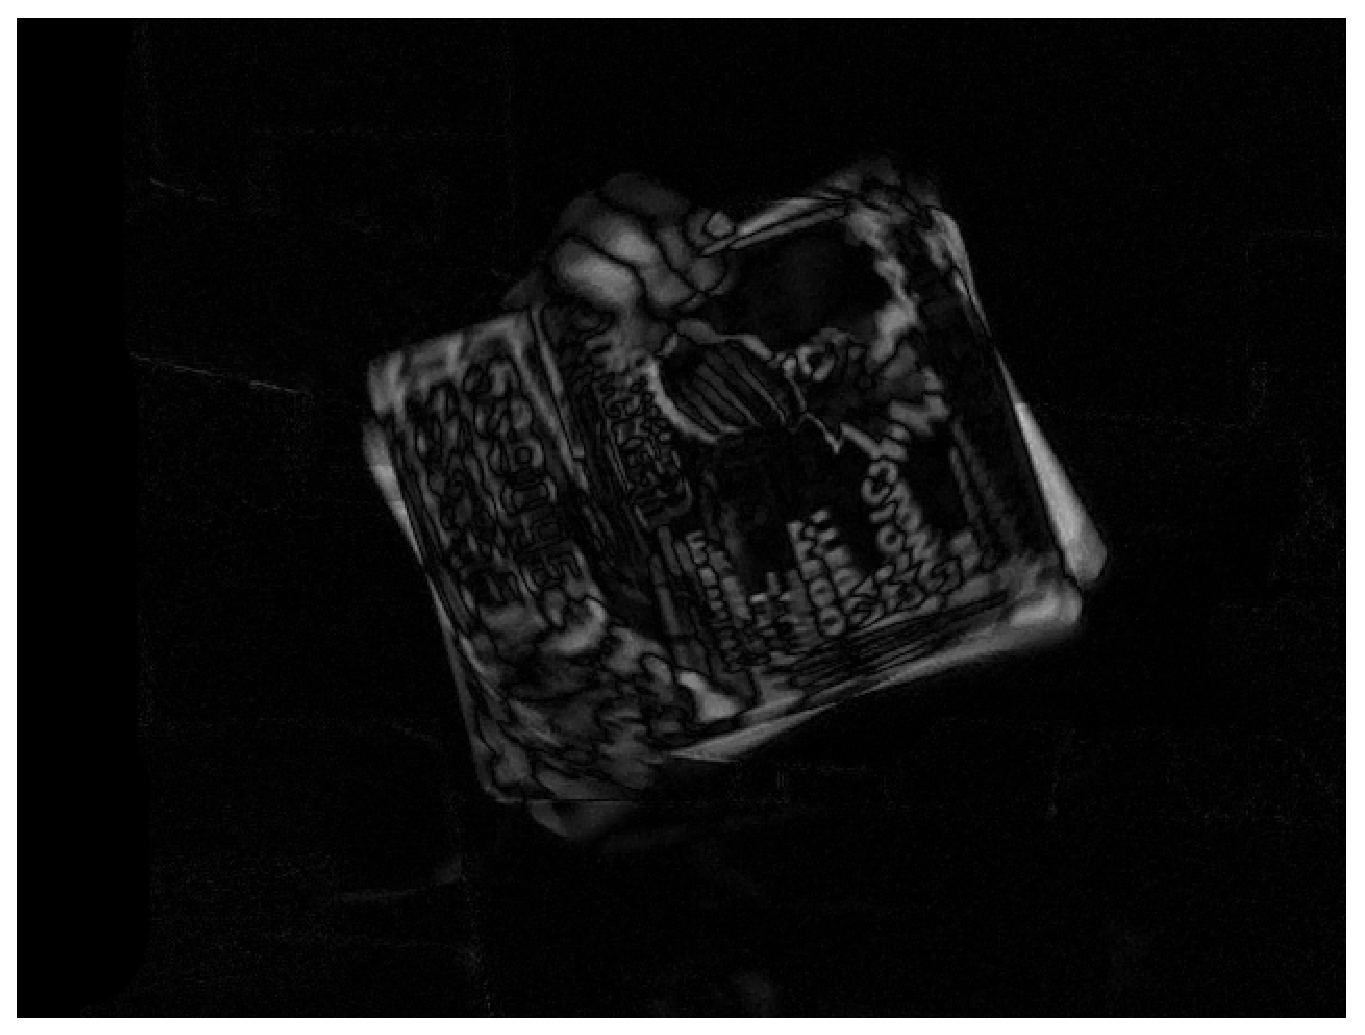
\includegraphics[width=0.27\textwidth]{../../figs/preprocess/absDiff} \label{fig:deteccion_movimietno-absdiff}}
    \subfloat[][\small{Umbral binario}]{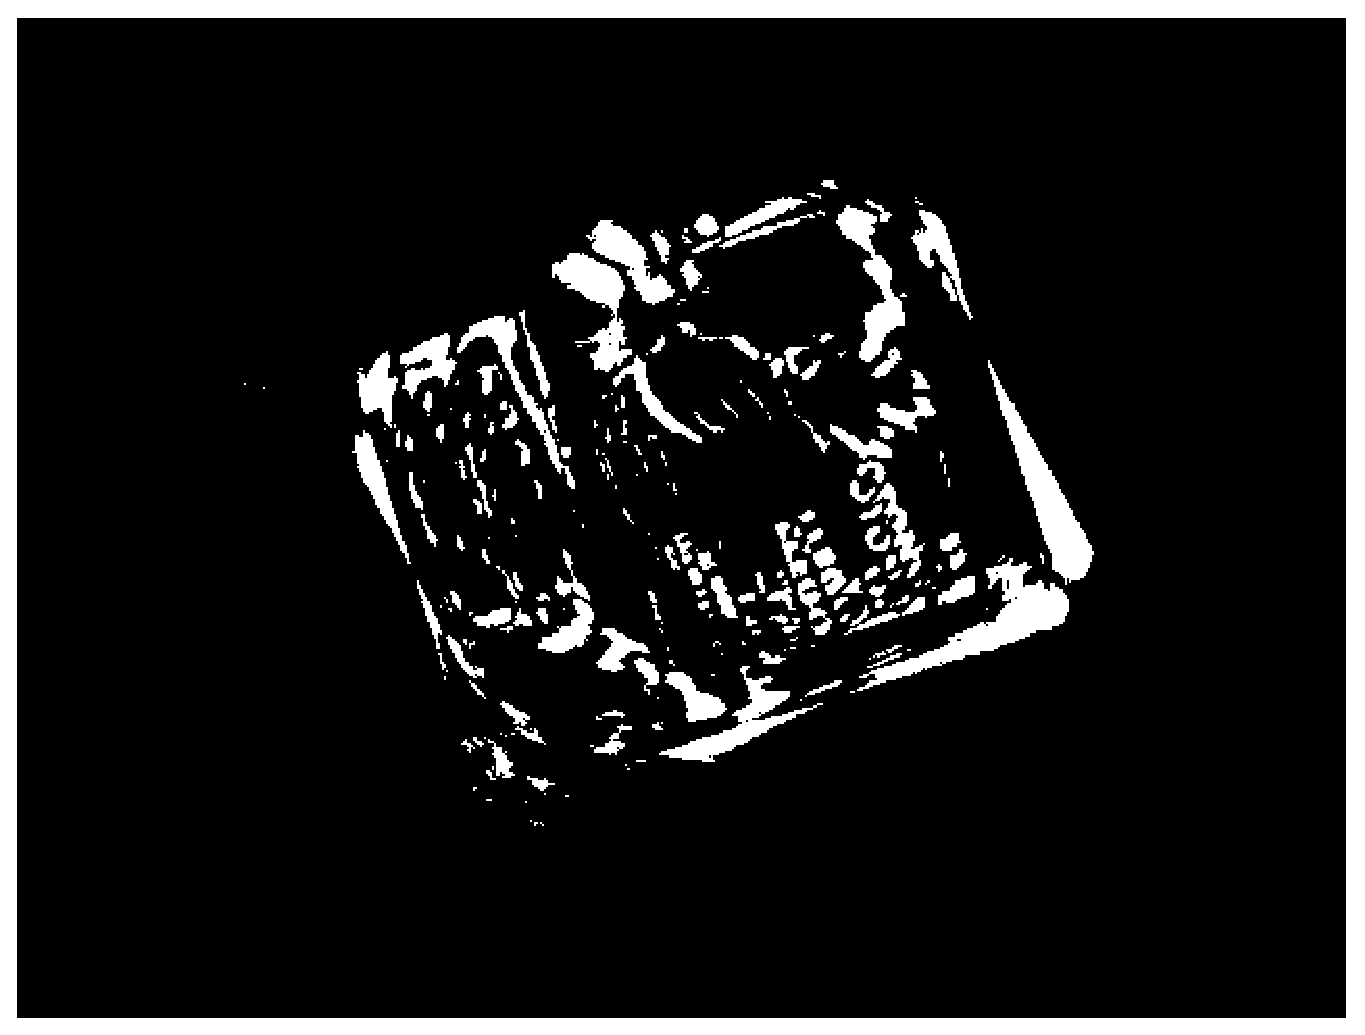
\includegraphics[width=0.27\textwidth]{../../figs/preprocess/threshold} \label{fig:deteccion_movimietno-umbral}}\\
    \subfloat[][\small{Erosión $\times2$}]{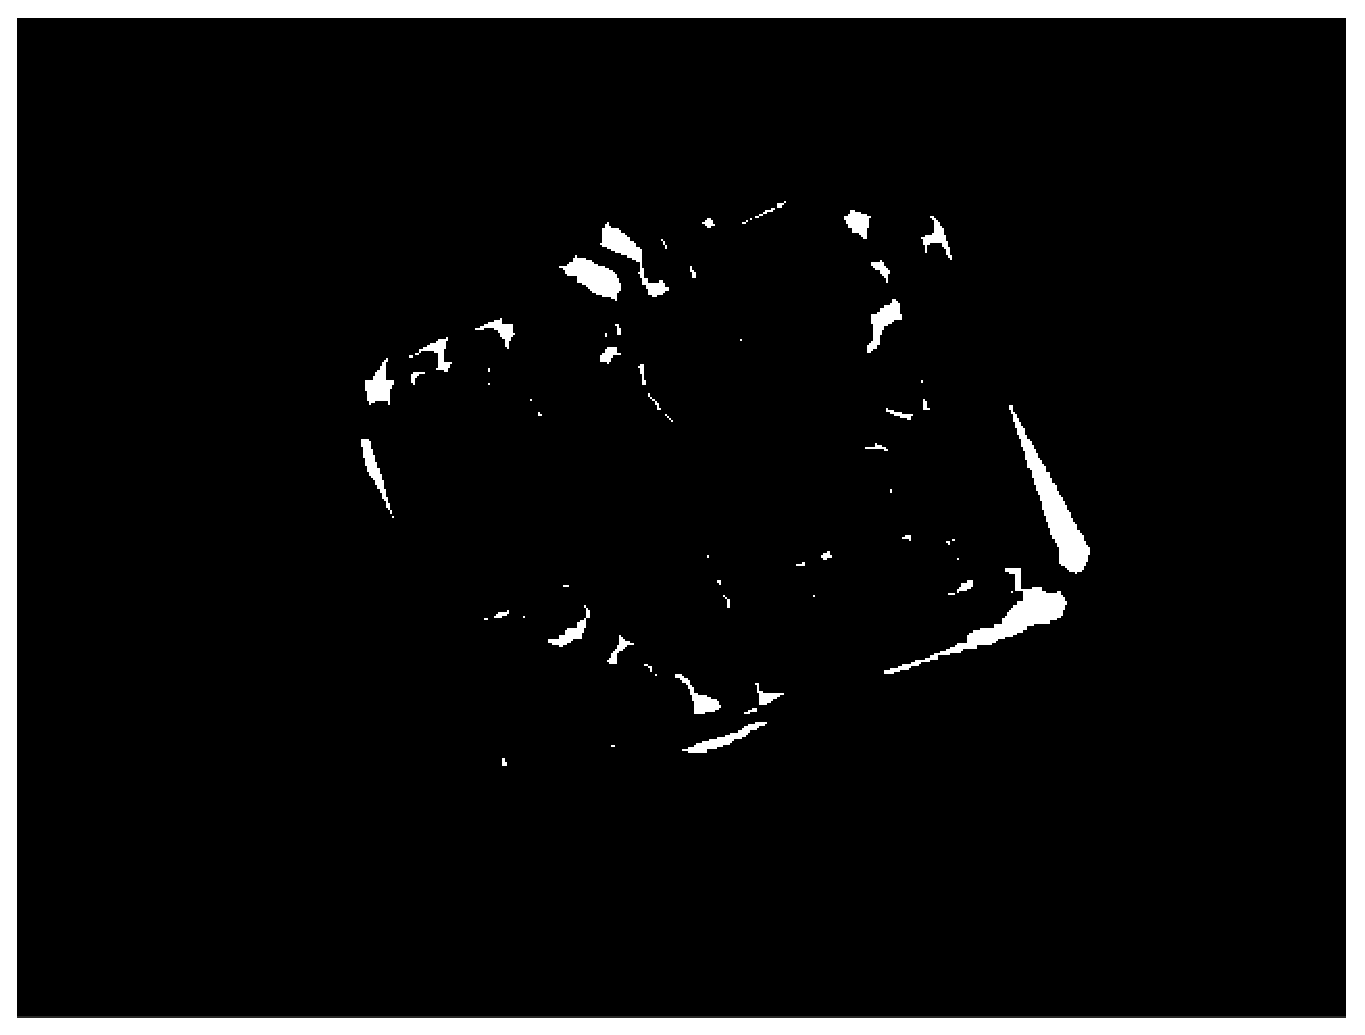
\includegraphics[width=0.27\textwidth]{../../figs/preprocess/erode} \label{fig:deteccion_movimietno-erode}}
    \subfloat[][\small{Dilatación $\times2$}]{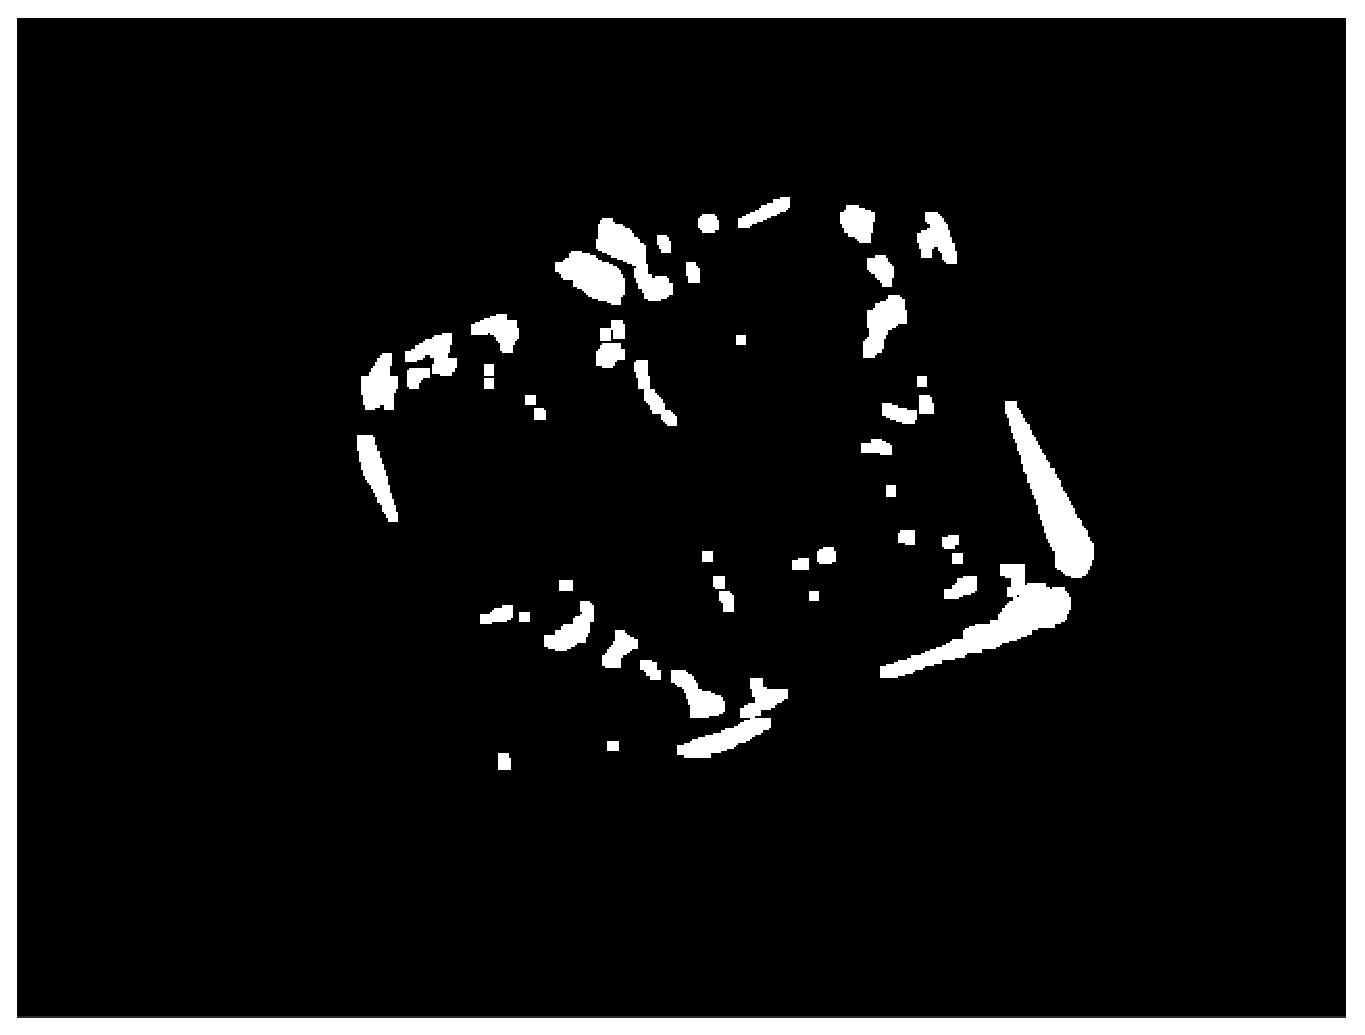
\includegraphics[width=0.27\textwidth]{../../figs/preprocess/dilate} \label{fig:deteccion_movimietno-dilate}}
    \subfloat[][\small{BR}]{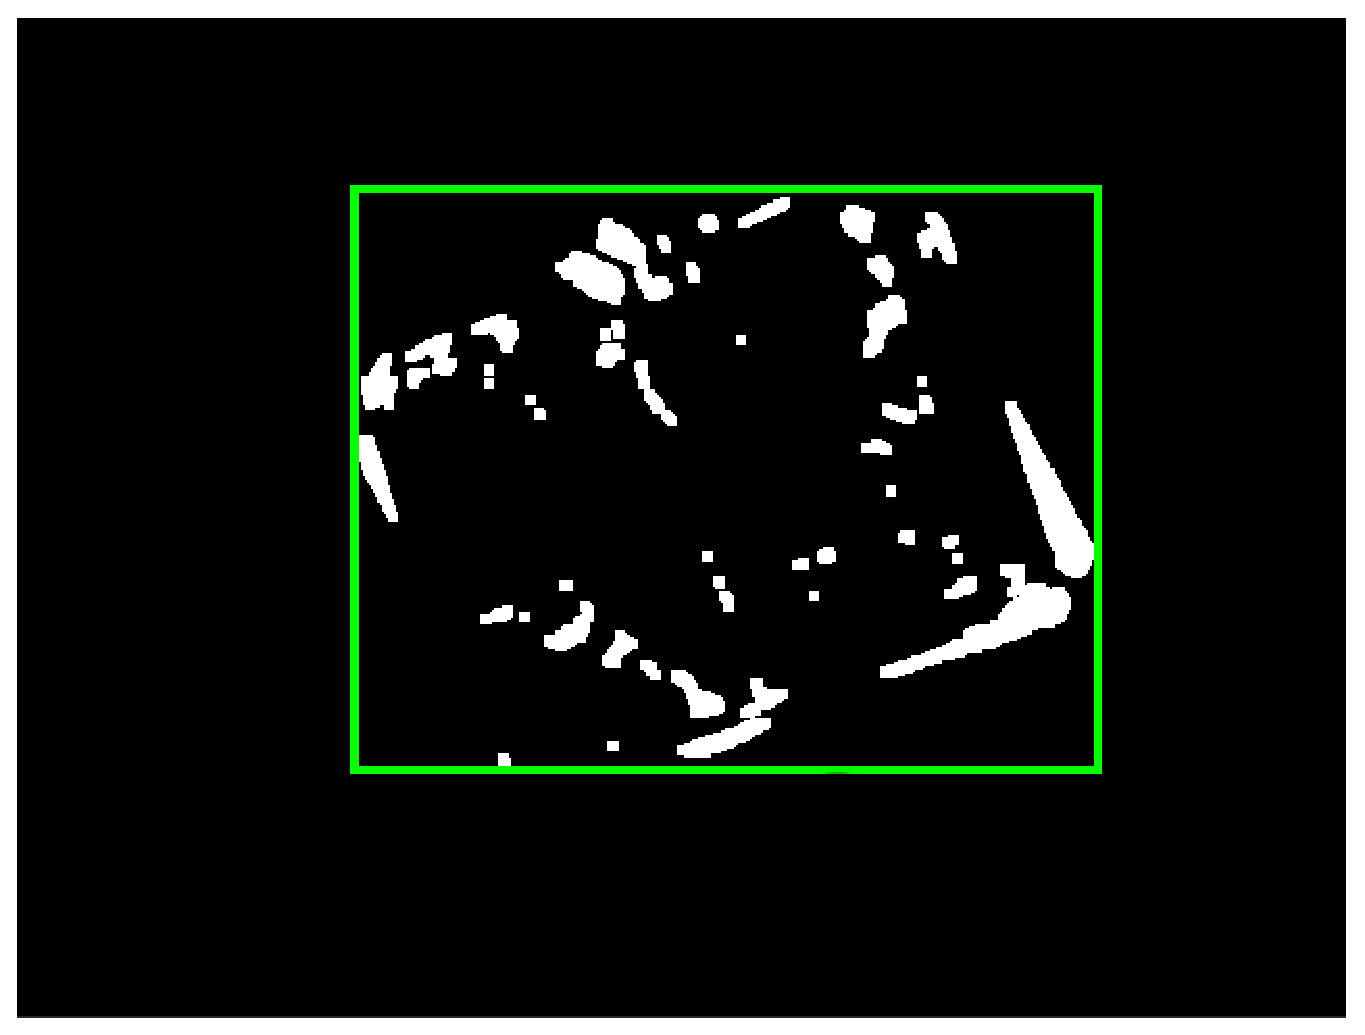
\includegraphics[width=0.27\textwidth]{../../figs/preprocess/boundingrect} \label{fig:deteccion_movimietno-boundingrect}}
    \caption[\small{Detección de movimiento}]{\small{Resultado de los procesos aplicados para la detección de movimiento.}}
    \label{fig:deteccion_movimiento}               %% Etiqueta para la figura entera
  \end{figure}
\end{frame}

% ver si pongo esto o no!!??
% \begin{frame}{Área de BR}
%  Si el area de BR > 10000 píxeles se continua con el proceso, sino se deriva
% \end{frame}

\subsection{Extracción de Características}
  %ver el tema de noctaves, noctaveLayers y hessianThreshold -> como no lo pongo me parece que lo debería mencionar
  \begin{frame}{Detección de puntos claves y descriptor}
      \begin{block}{\textbf{SURF} (Detector rápido de características robustas)}
	\begin{itemize}
	      \item Detector y descriptor de puntos claves.
		  \note[item]{blob detection refers to mathematical methods that are aimed at detecting regions in a digital image that differ in properties, such as brightness or color, compared to areas surrounding those regions. Informally, a blob is a region of a digital image in which some properties are constant or vary within a prescribed range of values; all the points in a blob can be considered in some sense to be similar to each other.}
	      \item Basado en \textbf{SIFT} (Transformación de características invariante a la escala).
	      \item Gran velocidad de cálculo (más rápido que SIFT) con tolerable pérdida de robustez. %(No está basados en kernels de punto flotante)
	\end{itemize}
      \end{block}
  \end{frame}
 %
 \begin{frame}{El problema de cambio de escala en correspondencias de puntos}
    \begin{itemize}
      \item Los objetos fotografiados a diferentes distancias, aparecen de diferente tamaños.
	  \note[item]{Si tomamos varias fotografias de un objeto a diferentes distancias, el objeto aparecerá de diferente tamaño}
      \item Buscar correspondencias utilizando un número fijo de píxeles vecinos $\rightarrow$ las intensidades no coincidirán.
	  \note[item]{Luego, si se tratan de buscar correspondencias entre las imágenes del objeto usando un tamaño FIJO de píxeles vecinos, la intensidad no coincidirá debido al cambio de escala presenten en las mismas y por lo tanto el reconocimiento fallará.}
      \item Definir un área vecina al punto clave con la misma información visual.
	  \note[item]{La escala define un área vecina con la misma información visual.
		  La motivación de generar una representación espacio escala se origina en que los objetos reales están compuestos por diferentes estructuras a diferentes escalas. Dependiendo de la escala de observación aparecen de diferentes tamaños. Por ejemplo el concepto de un árbol es apropiado a la escala de metros, pero el concepto de hojas o moléculas son apropiados para escalas más finas.}
    \end{itemize}
	    \note[item]{Si la escala del filtros gaussiano es muy pequeña, el resultado incluye muchos puntos redundantes de detalles innecesarios}
		\note[item]{Contrariamente, si la escala es muy grande, los puntos de regiones con soporte pequeño tienen a desaparecer con el borroneado}
		\note[item]{Para solucionar los problemas existentes en el filtrado gaussiano con escalas fijas, se han propuesto procedimientos espacio-escala basados en la representación de la curvatura discreta multi escalar}
 \end{frame}

 \begin{frame}
      \begin{block}{SURF}
	\begin{itemize}
	      \item Invariante a escala: asigna un factor de escala a cada punto clave.
		\note[item]{mediante el calculo del laplaciano usando filtros gaussianos a diferentes escalas.}
		\note[item]{La localización de los puntos se realiza mediante una interpolación con una función cuadrática. Esto se hace porque en filtros de tamaños grandes, el muestreo es grande y esto en la imágen representan a largas distancias respecto de la imagen base por asi decirlo}
	      \item Invariante a rotación: asigna una orientación a cada punto clave.
		  \note[item]{Asigna una orientación a cada punto detectado}
	      \item Determinante de la matriz hessiana para la determinación de la localización y escala de los puntos $\rightarrow$ umbral
		  \note[item]{puntos que superan un umbral son extraídos}
	      \item Vector descriptor $N$ dimensional (64 elementos) para cada punto clave.
		  \note[item]{La región es dependiente de la escala en que fue detectado el punto!!!}
		  \note[item]{$\rightarrow$ posibles de comparar con una métrica de distancia}
		  \note[item]{Región centrada en el punto clave (de tamaño dependiente de la escala) y en orientada de acuerdo a la orientación detectada anteriormente sobre la que se realizan diversas operaciones}
	      \item Cuanto más similares sean 2 puntos característicos más cercanos serán sus descriptores.
		  \note[item]{describe cómo las intensidades de los píxeles se distribuyen dentro de una vecindad, que es dependiente de la escala de cada punto de interés detectado por el hessiano}
		  \note[item] {Cuando el determinante del hessiano es un máximo local (previa eliminación de mínimos mediante un umbral), se determina un punto clave. El uso del hessiano es alentado por su velocidad de cálculo y precisión.
		  \begin{equation*}
		    H(x,y)=\begin{bmatrix}\frac{\partial^{2}I}{\partial x^{2}} & \frac{\partial^{2}I}{\partial x\partial y}\\
		    & \\
		    \frac{\partial^{2}I}{\partial y\partial x} & \frac{\partial^{2}I}{\partial y^{2}}
		    \end{bmatrix};\; \textrm{con}\; \frac{\partial^{2}I}{\partial x\partial y}=\frac{\partial^{2}I}{\partial y\partial x}.
		    \label{eq:HessianMatrix}
		  \end{equation*}
		  Sea $\mathbf{p}=(x,y)$ un punto en la imagen $\mathit{I}$
		  la matriz hessiana en $\mathbf{p}$ en la escala $\sigma$ viene definida como:
		  \begin{equation*}
		    \mathcal{H}(\mathbf{p},\sigma)=\left[\begin{array}{cc}
		    \mathit{L_{xx}(\mathbf{p},}\sigma)\hphantom{} & \mathit{L_{xy}(\mathbf{p},}\sigma)\\
		    \mathit{L_{xy}(\mathbf{p},}\sigma)\hphantom{} & \mathit{L_{yy}(\mathbf{p},}\sigma)
		    \end{array}\right],
		  \end{equation*}
		  $\mathit{L_{xx}(\mathbf{p},}\sigma)$ es la convolución de la derivada segunda de una gaussiana $\frac{\partial^{2}}{\partial x^{2}}\mathit{g}(\sigma)$ con la imagen $\mathit{I}$ en el punto $\mathbf{p}$
		  }
		  \note[item]{$\mathit{L_{xx}(\mathbf{p},}\sigma)$ es la convolución de la derivada segunda de una gaussiana $\frac{\partial^{2}}{\partial x^{2}}\mathit{g}(\sigma)$ con la imagen $\mathit{I}$ en el punto $\mathbf{p}$}
		  \note[item]{$\mathit{L_{xy}(\mathbf{p},}\sigma)$ es la convolución de la derivada segunda de una gaussiana $\frac{\partial^{2}}{\partial x \partial y}\mathit{g}(\sigma)$ con la imagen $\mathit{I}$ en el punto $\mathbf{p}$}
		  \note[item]{$\mathit{L_{yy}(\mathbf{p},}\sigma)$ es la convolución de la derivada segunda de una gaussiana $\frac{\partial^{2}}{\partial y^{2}}\mathit{g}(\sigma)$ con la imagen $\mathit{I}$ en el punto $\mathbf{p}$.}
	\end{itemize}
      \end{block}
  \end{frame}
% \begin{frame}{SURF}
% % 	  \begin{figure}[tbhp]
% % 	    \centering
% % 		  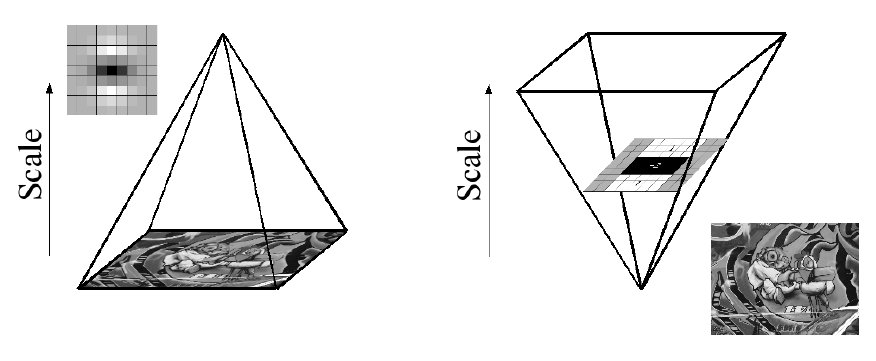
\includegraphics[scale=0.41]{../../figs/pyramidfilters}
% % 	      \caption[Pirámide de escala de imágenes para SIFT y SURF]{Pirámide de escala de imágenes para el método SIFT (izquierda) y el método SURF (derecha).}
% % 	    \label{fig:pyramidfilters}          %% Etiqueta para la figura entera
% % 	  \end{figure}
% 
% 	  %aclarar el tema de los box filters y de las imagenes integrales
% 	       
% 	       \begin{figure}[tbhp]
% 		  \centering
% 		  %%----primera subfigura----
% 		  \subfloat[]{
% 			\label{fig:gaussiankernelsdiscreted_y}         %% Etiqueta para la primera subfigura
% 			\includegraphics[scale=0.3]{../../../img_ent2/gaussiankernelsdiscrete_y}}
% 			\hspace{0.1\linewidth}
% 		  %%----segunda subfigura----
% 		  \subfloat[]{
% 			\label{fig:gaussiankernelsaprox_y}         %% Etiqueta para la segunda subfigura
% 			\includegraphics[scale=0.3]{../../../img_ent2/gaussiankernelsaprox_y}}
% 			\hspace{0.1\linewidth}
% 		  %%----tercera subfigura----
% 		  \subfloat[]{
% 			\label{fig:gaussiankernelsdiscreted_xy}         %% Etiqueta para la segunda subfigura
% 			\includegraphics[scale=0.3]{../../../img_ent2/gaussiankernelsdiscrete_xy}}
% 			\hspace{0.1\linewidth}
% 		  %%----cuarta subfigura----
% 		  \subfloat[]{
% 			\label{fig:gaussiankernelsaprox_xy}         %% Etiqueta para la segunda subfigura
% 			\includegraphics[scale=0.3]{../../../img_ent2/gaussiankernelsaprox_xy}}
% 			\hspace{0.1\linewidth}
% 		\caption[\scriptsize{Derivadas parciales gaussianas discretas y aproximadas}]{\scriptsize{Derivadas parciales gaussianas de segundo orden discretas y sus homólogas aproximadas (también referenciadas como filtros tipo caja). Las regiones grises de la imagen son iguales a cero.}}%% Etiqueta para la figura entera
% 		  \label{fig:gaussiankernels}
%       \end{figure}
%       SURF utiliza filtros aproximados (Box filters) \note[item]{combinado con el uso de imágenes integrales, se calcula más rápidamente}
% 	  \note[item]{Así el determinante de la matriz hessiana (aproximado) usado por SURF queda definido como:}
% 	  \begin{equation*}
% 	    \label{eq:det_happrox}
% 	    \det(\mathcal{H}_{approximado})=D_{xx}D_{yy}-(wD_{xy})^{2} 
% 	  \end{equation*}
% 	  con $w=0.9$ y donde $\mathit{D}_{xx}$, $\mathit{D}_{yy}$ y $\mathit{D}_{xy}$ son las derivadas parciales gaussianas de segundo orden aproximadas.
% 	  \note[item]{ La ponderación relativa $w$ de la respuesta del filtro es usada para balancear la expresión del determinante hessiano. Si bien el mismo varía para diferentes escalas, en la práctica se puede establecer este factor como constante con $w=0.9$, ya que el mismo no tiene un impacto significante en los resultados}
% \end{frame}

% \begin{frame}{SURF}
%   \begin{block}{Puntos claves}
% 	\begin{itemize}
% 	    \item Asigna un factor de escala a cada punto clave detectado.
% 	    \item La escala define un área vecina con la misma información visual
% 	    \item Asigna una orientación a cada punto detectado 
% 	\end{itemize}
%   \end{block}
% 
%   \begin{block}{Descriptores}
%       \begin{itemize}
% 	\item Región centrada en el punto clave (de tamaño dependiente de la escala) sobre la que se realizan diversas operaciones
% 	\item Se crea un vector N dimensional (64 elementos) por cada punto clave $\rightarrow$ posibles de comparar con una métrica de distancia,
% 	\item Cuanto más similares sean 2 puntos característicos más cercanos serán sus descriptores.  
%       \end{itemize}
%   \end{block}
% \end{frame}

% \begin{frame}{El problema de cambio de escala en correspondencias de puntos}
%  \begin{itemize}
%   \item Tener un factor de escala asociado con cada punto detectado.
%   \item Calculo del laplaciano de un punto en una imagen usando filtros gaussianos a diferentes escalas.
%     \note[item]{Si la escala del filtros gaussiano es muy pequeña, el resultado incluye muchos puntos redundantes de detalles innecesarios}
%     \note[item]{Contrariamente, si la escala es muy grande, los puntos de regiones con soporte pequeño tienen a desaparecer con el borroneado}
%     \note[item]{Para solucionar los problemas existentes en el filtrado gaussiano con escalas fijas, se han propuesto procedimientos espacio-escala basados en la representación de la curvatura discreta multi escalar}
%     \note[item]{El esquema está basado en el criterio de estabilidad que establece que la presencia de una esquina debe ocurrir como un máximo de curvatura observable en la mayoría de las escalas} %\cite{springerlink:10.1023/A:1008045108935}
%   \item Mediante las respuestas para diferentes escalas, se obtiene una curva que alcanza un valor máximo en algún valor de $\sigma$ (varianza de la función gaussiana) 	  \note[item]{$\sigma$ define implícitamente la escala en que la derivada es evaluada.}
%   \item Si se extrae este valor para dos imágenes del mismo objeto (tomadas a diferentes esclas), la relación que existe entre los $\sigma$ máximos se corresponderán en relación con las escalas en que fueron tomadas cada una de las fotografías.
%     \note[item]{Esta observación es el núcleo del proceso de extracción de características invariantes a la escala}
%  \end{itemize}
% \end{frame}

% \begin{frame}{Invarianza a escala}  
% 	\begin{center}
% 	    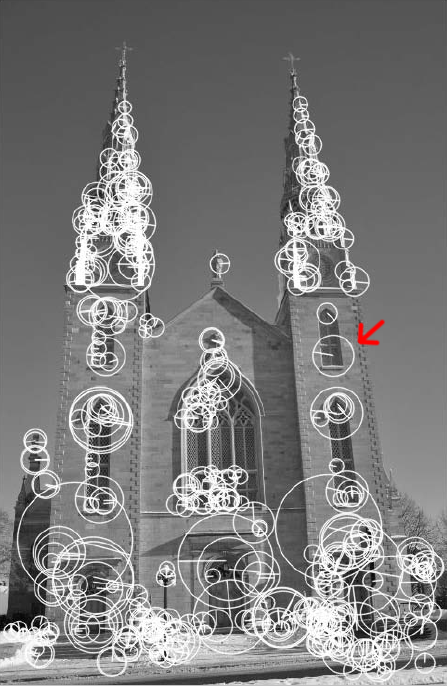
\includegraphics[scale=0.3]{./img1/surfinchurch1} \qquad
% 	    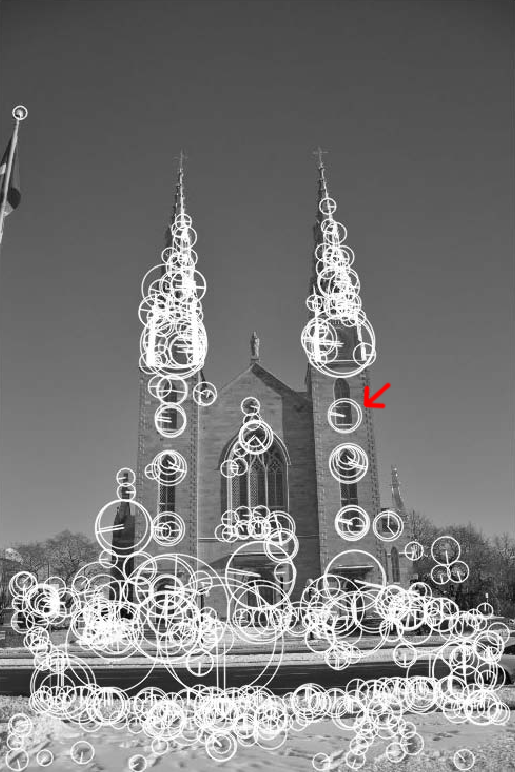
\includegraphics[scale=0.267]{./img1/surfinchurch2}
% 	\end{center}
% \end{frame}

%%%%%%%%%%%%%%%%%%%%%%%%%%%%%%%%%%%%%%%%%%%%%%%%%%%%%%%%%
\subsection{Correspondencia de puntos entre imágenes}
\begin{frame}{Búsqueda de correspondencias}
    \note[item]{calcular un valor que represente el grado de similitud de dos imágenes}
    \begin{block}{Grado de similitud}
    Grado de similitud entre vectores mediante distancia euclídea.
      \begin{itemize}
	\item NNS (Búsqueda del vecino más cercano).
	    \note[item]{Dado un conjunto de puntos $P=\left\{ p_{1,...,}p_{n}\right\}$ en un espacio métrico $M$ y un punto de consulta $q \in M$, encontrar el punto más cercano a $q$ en $P$ de forma eficiente, donde $M$ es un espacio euclídeo d-dimensional y la distancia es medida por ejemplo mediante la distancia euclídea.
	    }
	      \note[item]{$\root{(x_2-x_1)^2+(y_2-y_1)^2}$ - La distancia entre dos puntos es igual al módulo del vector que tiene de extremos dichos puntos.}
	      \note[item]{El módulo de un vector es la longitud del segmento orientado que lo define. $P=(3,4) entonces \root{3^2+4^2})$}
	\item $K$-NN (K vecinos más cercanos).
	  \note[item]{si $K=1$ $\rightarrow$ NNS}	
	\item Búsqueda aproximada mediante $KD$-tree o multiple $KD$-tree aleatorio.
	  \note[item]{Se usan 2 o 4 árboles examinándose todas las hojas (las 64) y buscando los 2 vecinos más cercanos}
	  \note[item]{Búsqueda aproximada del vecino más cercano $\rightarrow$ mejora los tiempos de ejecución con errores de precisión aceptables.}
	  \note[item]{
	    \begin{itemize}
	    \item KD-tree: 
		  \note[item]{Los elementos guardados en el árbol KD-tree, son vectores de altas dimensiones}
		  \note[item]{Para construir el árbol, se compara el vector de entrada con el ``valor de partición'' para determinar a qué mitad del árbol pertenece dicho vector. Cada una de las dos mitades de los datos es dividida de igual manera y en forma recursiva, para lograr crear un árbol binario completamente balanceado.}
		  \begin{itemize}
		      \item Creación de una estructura de árbol para la búsqueda 
			    \note[item]{En la raíz del árbol (primer nivel), los datos son divididos en dos mitades por un hiper plano ortogonal para una dimensión elegida y con un valor de umbral.}
			    \note[item]{Generalmente, esta división se realiza con la media, en la dimensión con la mayor varianza del conjunto de datos (para SIFT y SURF es la medida que presenta el mejor rendimiento)}
		      \item Eficiente con datos de bajas dimensiones
		  \end{itemize}
	    \item Múltiples árboles KD aleatorios \note[item]{Para acelerar la búsqueda}
	    \begin{itemize}
		  \item Búsqueda eficiente con datos de altas dimensiones
		      \note[item]{Los árboles aleatorios son construidos seleccionando la dimensión de división de forma aleatoria sobre las primeras $D=5$ dimensiones en las que los datos poseen mayor varianza.}
		      \note[item]{Cuando se realiza la b\'usqueda en el árbol, una cola con prioridad es mantenida a través de todos los arboles aleatorios, por lo que la búsqueda queda ordenada mediante el incremento de la distancia a cada nodo del borde.}
		      \note[item]{El grado de aproximación, se determina mediante el examen de un número fijo de nodos hoja.}
		      \note[item]{Cuando es alcanzado este número, se termina la búsqueda y se obtienen los candidatos.}
		  \item Se obtiene resultados aproximados
		  \item La cantidad de memoria utilizada aumenta
			\note[item]{Se debe tener en cuenta que la cantidad de memoria utilizada aumenta linealmente con el número de árboles aleatorios, una característica negativa cuya importancia no resulta menor en la sobrecarga del sistema.}
	      \end{itemize}
	    \end{itemize}
	}	
    \end{itemize}
  \end{block}
\end{frame}

\begin{frame}{Búsqueda de correspondencias}
  \begin{itemize}
  \item Cálculo de la distancia euclídea entre los vectores característicos.
    \note[item]{Las correspondencias son buscadas mediante el cálculo de la distancia euclídea entre los vectores característicos asociados a los puntos claves detectados en cada una de las imágenes.}
  \item Aplicación de un umbral para determinar las potenciales correspondencias válidas.
    \note[item]{se usa una relación entre el vecino más cercano y el segundo vecino más cercano}
%   \item Umbral global que se compare con la distancia a la característica más cercana no funciona correctamente
%   \note[item]{Usar un valor de umbral global que se compare con la distancia a la característica más cercana no funciona correctamente}
%   \item Se propone comparar la distancia del vecino más cercano ($d_1$) respecto del segundo vecino más cercano ($d_2$).
      \note[item]{$A$ y $B$ dos imágenes sobre las cuales se quieren buscar correspondencias}
      \note[item]{Consideremos $a_i$ con $i=0\ldots n$ un punto del conjunto de puntos claves detectados en $A$}
      \note[item]{$n$ el total de puntos claves detectados en $A$}
      \note[item]{$av_i$ el vector característico asociado al punto $a_i$}
      \note[item]{Para cada $a_i$, se seleccionan los dos mejores puntos claves candidatos $p_1 \in b_i$ y $p_2 \in b_i$ cuyos vectores de características asociados a cada uno representan las distancias euclídeas mínimas $d_1$ y $d_2$ respectivamente respecto a $av_i$}
%   \item Si $\frac{d_{1}}{d_{2}}>0.8$ la coincidencia es rechazada.
      \note[item]{con 0.6 es un poco más rápido pero menos estable}
      \note[item]{se puede interpretar como: si las dos coincidencias más cercanas no difieren por mucho, es un problema porque no sabemos cual de las dos es la correcta}
      \note[item]{Las coincidencias buenas necesitan tener el vecino más cercano, significativamente más cerca que las correspondencia mala}
      \note[item]{Aplicar un umbral global no funciona correctamente ya que algunos descriptores son más descriminativos que otros. Una medida más efectiva es usar la que usamos aquí: Muchas características de la imagen no tiene la correspondencia correcta en la imagen de entrenamiento ya que surgen de objetos del fondo por ejemplo. La idea es eliminar las características que no tienen una buena correspondencia.}
      \note[item]{El valor de $\varepsilon=0.8$ fue seleccionado de acuerdo al estudio llevado a cabo por Lowe que afirma que se alcanzan a eliminar un 90\% de falsas coincidencias mientras se descartan sólo un 5\% de buenas coincidencias, resultando en el valor más apropiado. Valores de $\varepsilon=0.6$ a $0.9$ también son apropiados.}
  \item Reducción de correspondencias espurias.
      \note[item]{Eliminar coincidencias espurias realza la habilidad de buscar la homografía correcta mediante la}
  \end{itemize}
\end{frame}
% \begin{frame}{Comparación}
% Encontrar correspondencias entre la imagen patrón y la imagen del flujo de video.
% 	\begin{itemize}
% 		\item Correspondencia de características entre imágenes
% 		\item Patrón buscado presente en imagen capturada? $\rightarrow$ Comparación de vectores característicos de imagen Patrón y Frame del flujo de video.
% 	\end{itemize}
% \end{frame}
% 
% \begin{frame}{Herramientas}
% 	\begin{itemize}	
% 		\item Métrica de distancia (euclídea, manhattan, etc.)
% 		\item Vectores de grandes dimensiones (NNS por fuerza bruta - lento).
% 		\item Variante para reducir tiempos: Multiples árboles aleatorios KD-tree.
% 		\item Retorna los mejores candidatos (aproximados)
% 	\end{itemize}
% \end{frame}
%%%%%%%%%%%%%%%%%%%%%%%%%%%%%%%%%%%%%%%%%%%%%%%%%%%%%%%%%

\subsection{Transformación y RA}
\begin{frame}{Transformación proyectiva - Homografía}
\note[item]{Marcelo: Transformación proyectiva !ojo! no es lo mismo imagen que el objeto y los puntos del objeto son los que buscamos.
}
 \begin{itemize}
  \note[item]{cvFindHomografphy: Se busca la transformación perspectiva entre dos planos}
  \item Relación proyectiva entre dos imágenes de una misma escena tomadas desde diferentes puntos de vista.
      \note[item]{Al tomar dos imágenes de una misma escena desde diferentes puntos de vista, existe una importante relación proyectiva entre éstas y la escena.}
      \note[item]{Una transformación proyectiva (también conocida con los términos equivalentes: colineación u homografía) es un mapeo invertible $h$ de $\mathbb{P}^2$ a sí mismo, de tal manera que tres puntos $x_1, x_2, x_3$ están sobre la misma línea si y solo si $h(x_1), h(x_2), h(x_3)$ también lo están. }
      %     \begin{block}{Transformación proyectiva}
      %       Un mapeo $h$: $\mathbb{P}^2 \rightarrow \mathbb{P}^2$ es una transformación proyectiva si y solo si existe una matriz de $3 \times 3$ ($\textit{H}$) tal que para cada punto en $\mathbb{P}^2$ representado por un vector $\mathbf{x}$ se cumple que $h(\mathbf{x})=\textit{H}(\mathbf{x})$. 
      %     \end{block}
      
  \item La relación entre las dos imágenes es una homografía si se cumple la ecuación $\textbf{x'}=H\textbf{x}$: 
      \note[item]{Si consideramos el conjunto de puntos $(x_i,y_i,z_i)$ perteneciente a una primer imagen y sabemos que mapean a un conjunto de puntos $(x'_i, y'_i, z'_i)$ en la segunda imagen (ambos en coordenadas homogéneas), la relación entre las dos imágenes es una homografía si se cumple la ecuación} %\eqref{eq:eq_cumple_homografia}.
      \begin{equation*}
	\begin{bmatrix}
	x'_i\\
	y'_i\\
	z'_i
	\end{bmatrix}=\textit{H}
	\begin{bmatrix}
	x_i\\
	y_i \\
	z_i
	\end{bmatrix}\Longrightarrow
      \begin{bmatrix}
	x'_i\\
	y'_i\\
	z'_i
	\end{bmatrix}=
	\begin{bmatrix}
	h_{11} & h_{12} & h_{13}\\
	h_{21} & h_{22} & h_{23}\\
	h_{31} & h_{32} & h_{33}\\
	\end{bmatrix}
      \begin{bmatrix}
	x_i\\
	y_i \\
	z_i
	\end{bmatrix}.
	\label{eq:eq_cumple_homografia}
      \end{equation*}
      \item Los puntos en una vista pueden ser convertidos a la segunda vista mediante $H$.
	\note[item]{Una vez que se a logrado obtener $\textit{H}$, todos los puntos en una vista pueden ser convertidos a la segunda vista usando esta relación.}
	\note[item]{Dos Fotografías de diferentes puntos de vista (imagen patrón y frame de flujo de video).}
	\note[item]{En qué lugar un punto en una fotografía se encuentra en la otra $\rightarrow$ Matriz homográfica.}
	\note[item]{Busca la transformación perspectiva entre dos planos. $x'=Hx$}
  \end{itemize}
\end{frame}

\begin{frame}{Estimación de $H$}
\note[item]{La homografía transformación proyectiva u homografía, es la proyección perspectiva entre dos imágenes y es derivada de las posiciones de los puntos claves en la imagen patrón y los puntos coincidentes detectados en la imagen objetivo.}
  \begin{itemize}
  \item Se pueden tener pares de correspondencias que no son válidos o tener más de 4 pares de correspondencias necesarios para calcular $H$.
      \note[item]{Un punto $2D$ $(x,y)$ en una imagen es representado por un vector $3D$ $\textbf{x}=(x_1,x_2,x_3)$ donde $x=\frac{x_1/x_3}$ y $y=\frac{x_2/x_3}$. Esto es llamado representación homogénea de un punto y se encuentra sobre el plano proyectivo $P^2$. Se debe notar que $H$ puede cambiar multiplicandose por una constante arbitraria no cero sin alterar la transformación proyectiva. Es decir que $H$ es considerada una matriz homogénea y tiene solo 8 grados de libertad a persa de contener 9 elementos. Es decir que hay 8 incógnitas que se tienen que resolver.}
      \note[item]{La transformación proyectiva u homografía es una transformación lineal no singular de coordenadas homogéneas: transformación lineal que tiene inversa}
      \note[item]{¿¿Cuáles pares coinciden con la estimación?}
      \note[item]{Cuatro pares son necesarios para estimar la homografía}
      \note[item]{en cuyo caso la matriz $\textit{H}$ puede resultar incorrecta}
  \item Se procede mediante una estimación de la homografía.
      \note[item]{Determinar la ``mejor'' transformación a partir de los datos, lo cual se convierte en la búsqueda de la transformación $\textit{H}$ que minimice una función de costo.}
  \item RANSAC (\textit{random sample consensus}) puede hallar la mejor solución aproximada minimizando el error y depurando coincidencias válidas y espurias iterativamente.
      \note[item]{Además usa más de cuatro correspondencias lo que logra una mejor estimación. Minimiza el error de reproyección creo que 5 píxeles de error?}
      \note[item]{No se utiliza LMEDS porque necesita tener certeza que hay 50\% de valores exactos}
      \note[item]{Las correspondencias deben ser lo suficientemente buenas.}
      \note[item]{Aplicación de la Matriz homográfica a la imagen a sobre imponer sobre el objeto detectado (RA)}
  \end{itemize}
\end{frame}

% \begin{frame}{Homografía}  
%   \begin{figure}[tbhp]
%     \centering
% 	  \includegraphics[scale=0.5]{../../figs/transfperspectiva}
%       \caption[Esquema de transformación perspectiva]{Esquema de transformación perspectiva utilizando la homografía $H$.}
%     \label{fig:transf_pespectiva}
%   \end{figure}
% \end{frame}

% \begin{frame}{Homografía - Detección}
%   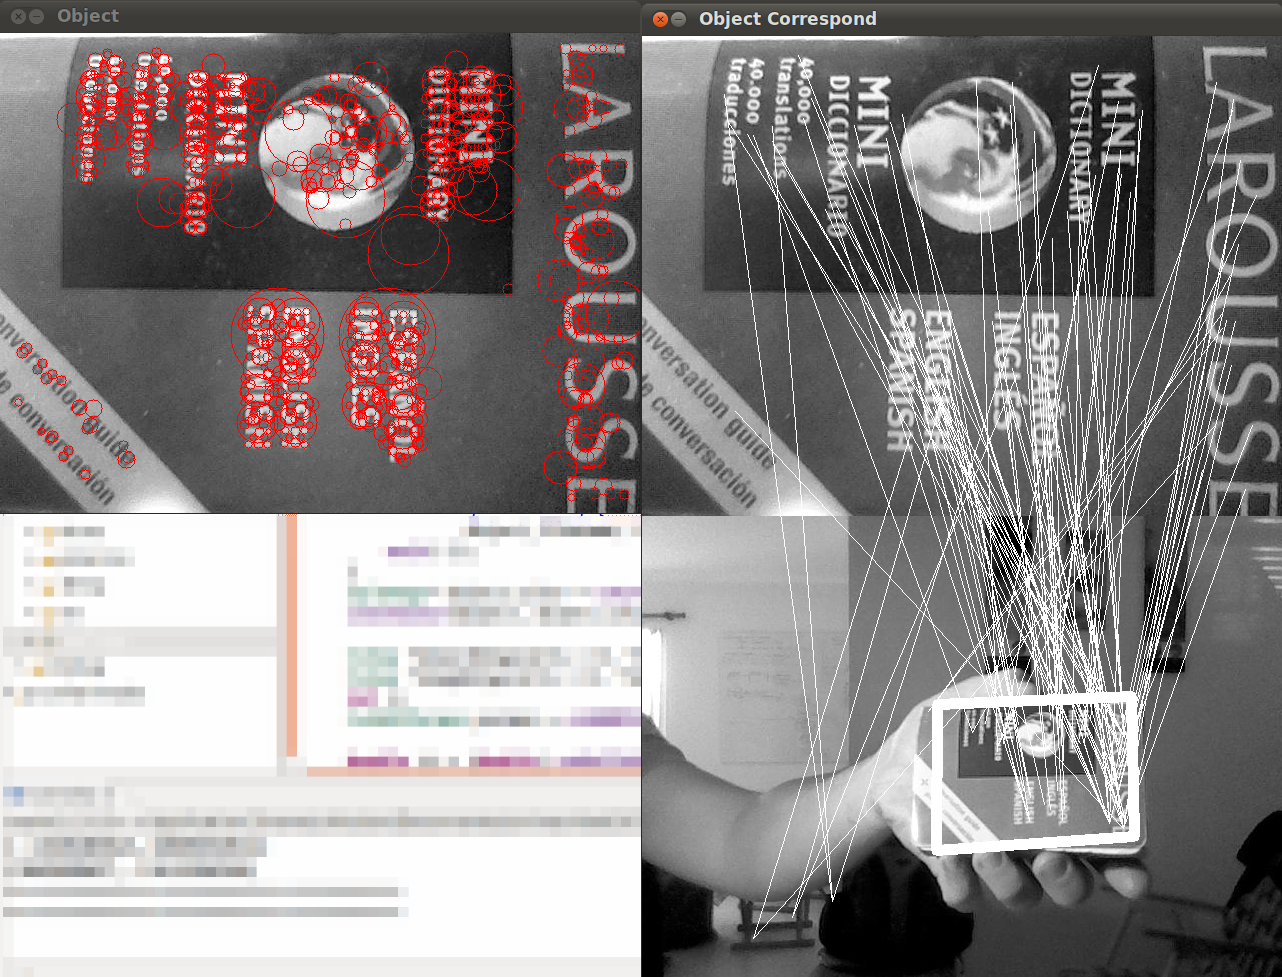
\includegraphics[scale=0.2]{./img1/correspo1}
% \end{frame}

\begin{frame}{Homografía - Detección}
  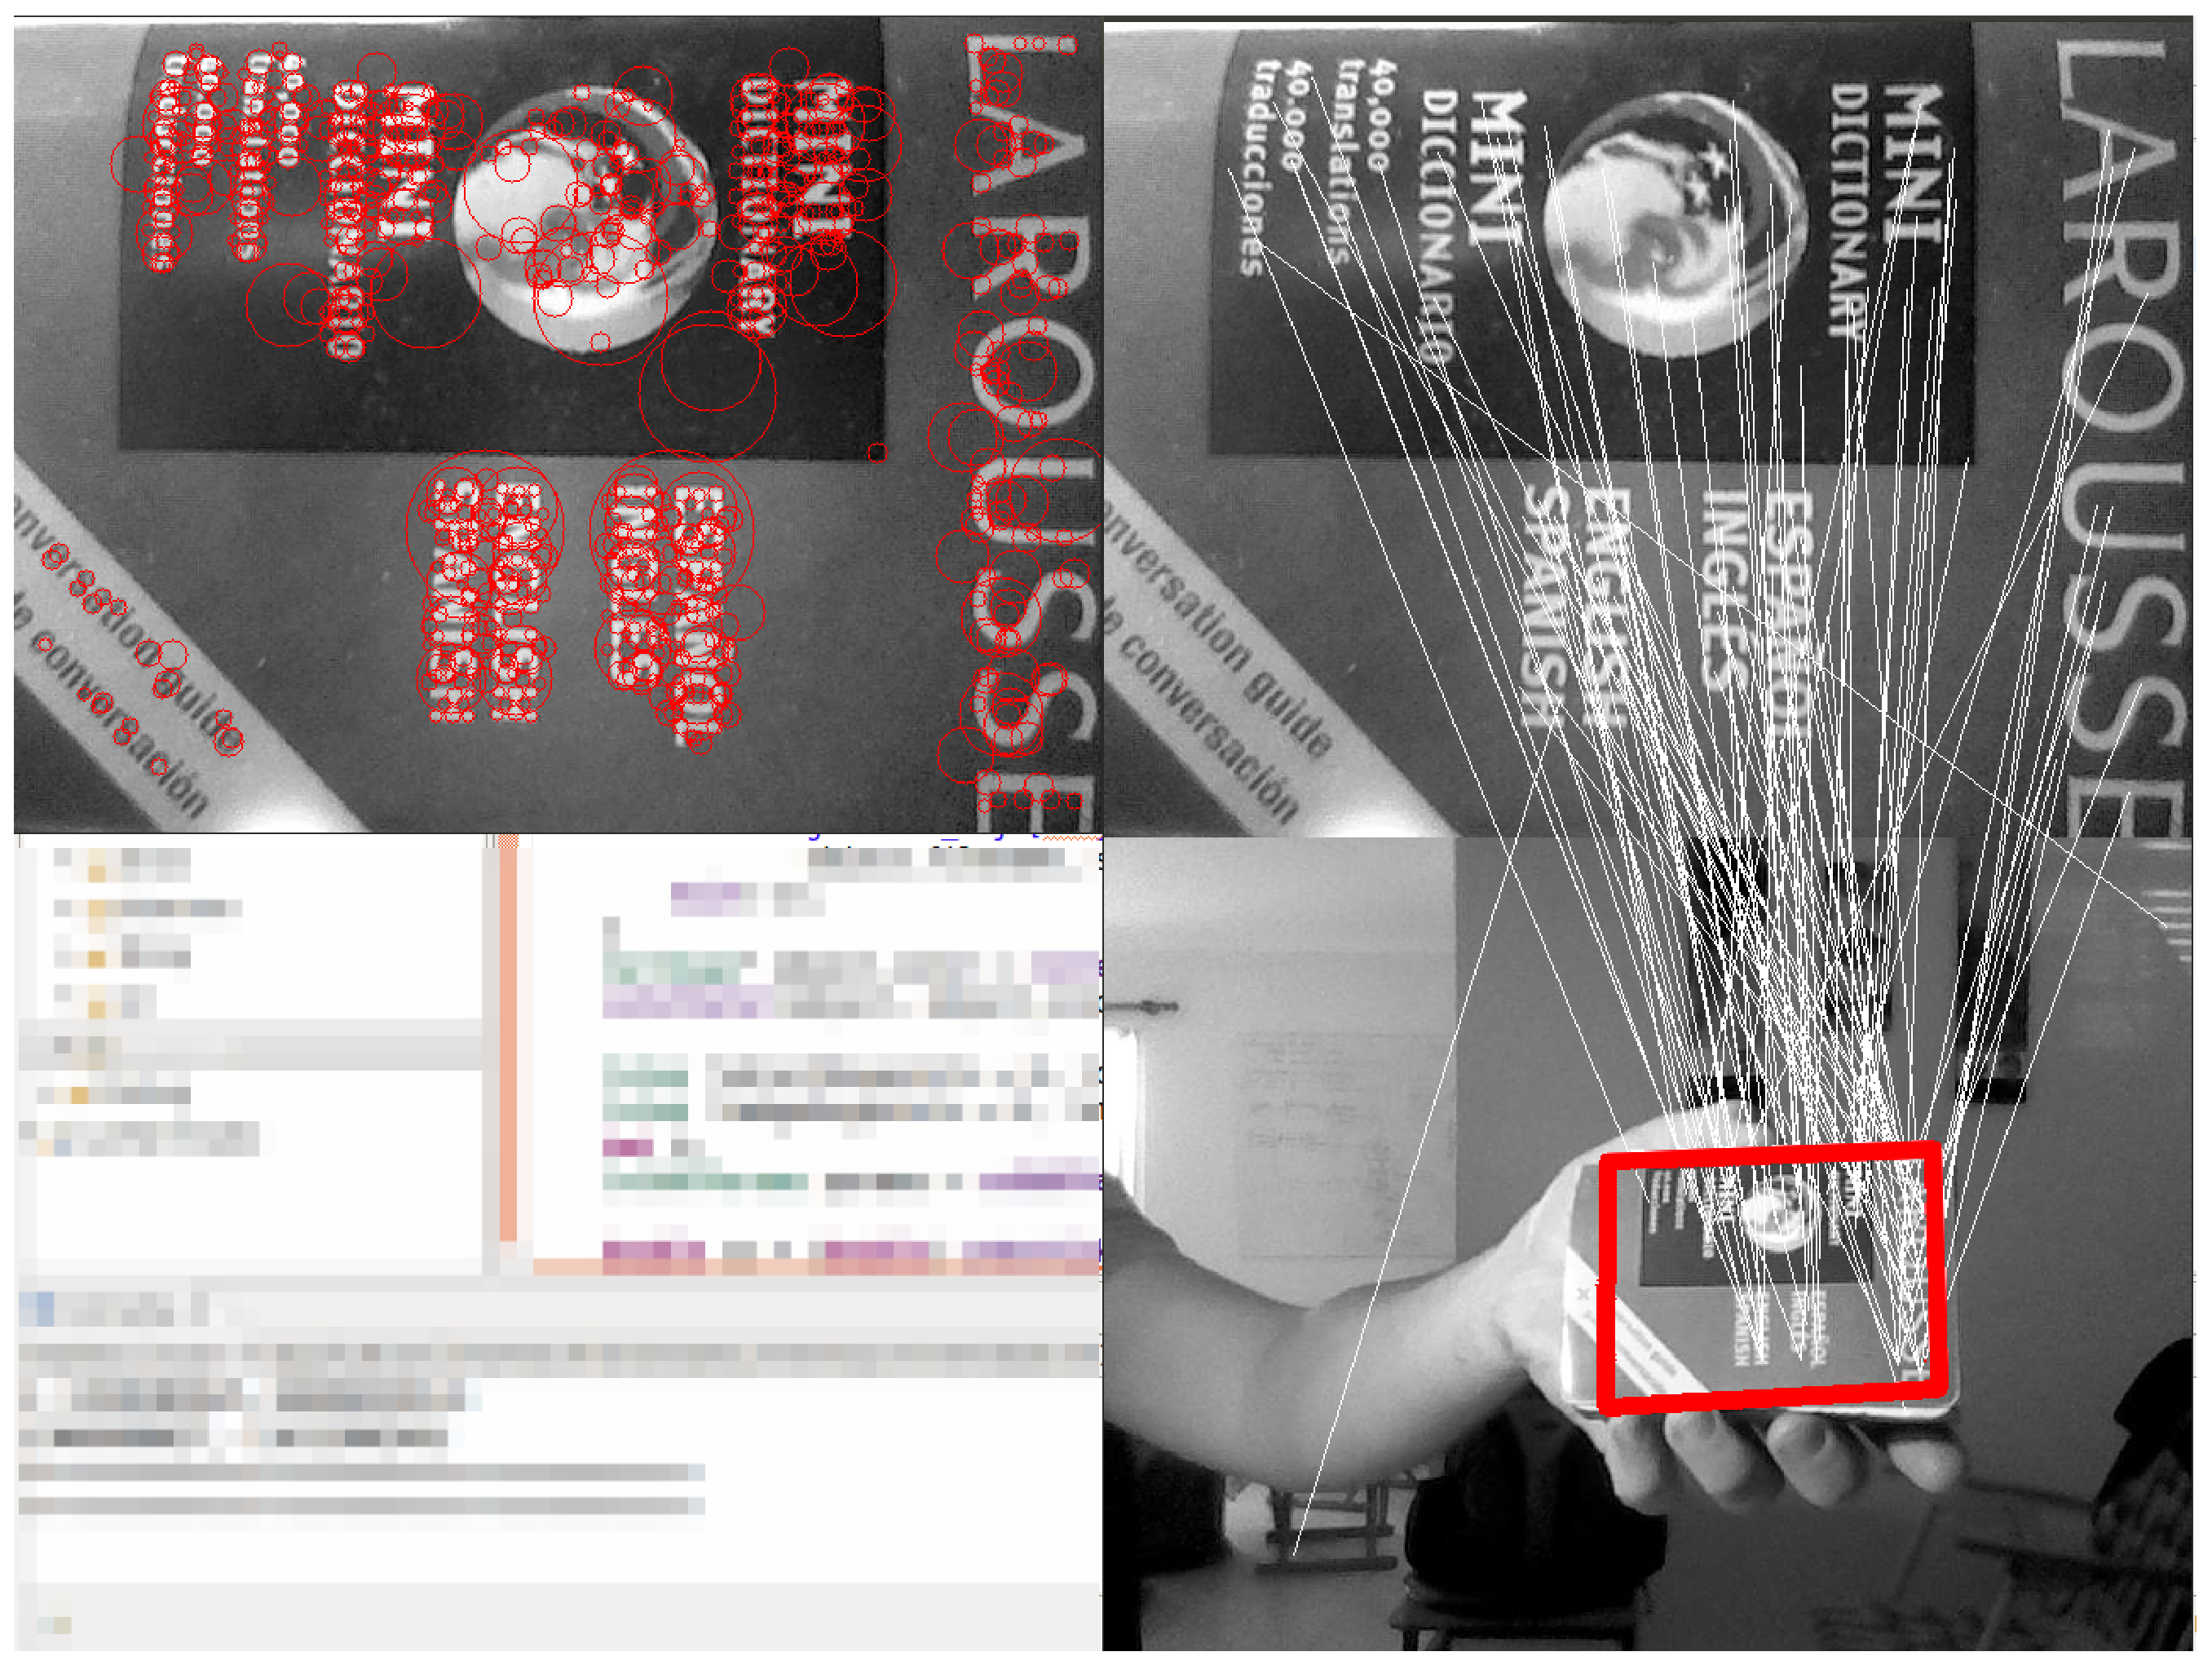
\includegraphics[scale=0.2]{./img1/correspo2_color}
    \note[item]{Explicar lo que es el recuadro rojo.}
    \note[item]{Marcelo: explicar que es lo que se vé en la imagen}
    \note[item]{Marcelo: Decir que son los círculos rojos}
\end{frame}

\begin{frame}{Homografía - Detección fallida}
  \note[item]{Explicar lo que es el recuadro rojo.}
  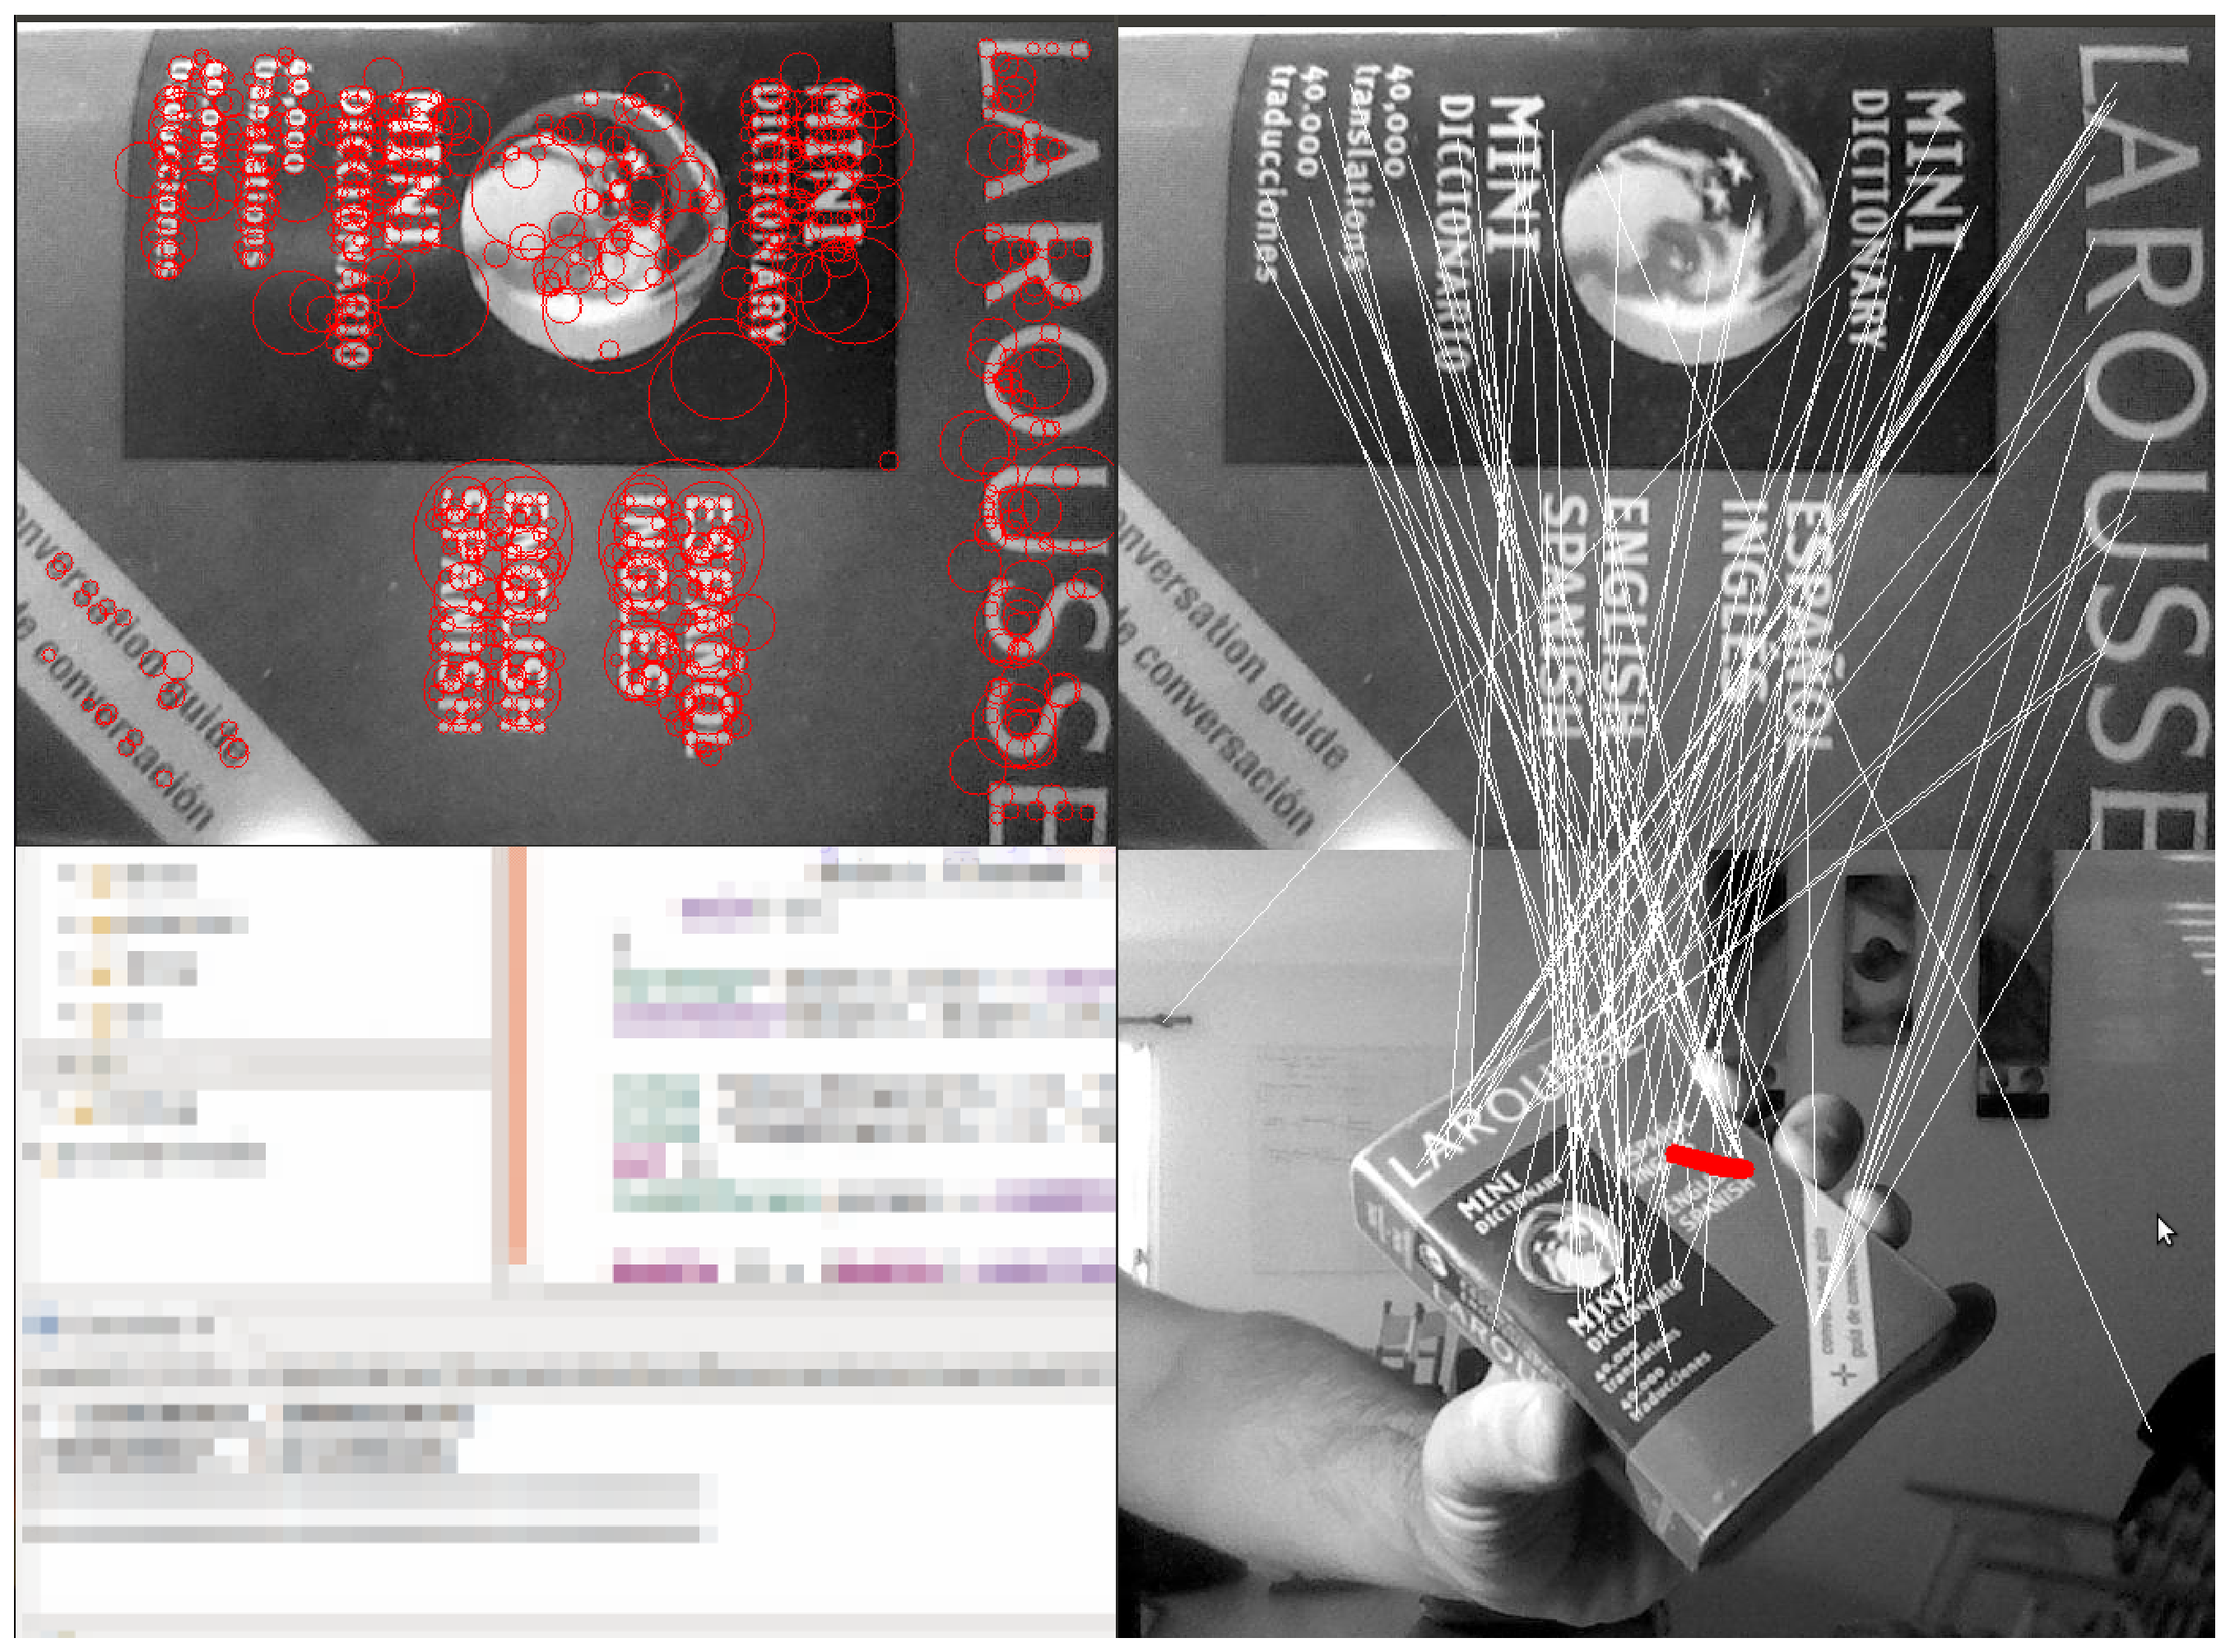
\includegraphics[scale=0.2]{./img1/correspo3_color}
\end{frame}

%%%%%%%%%%%%%%%%%%%%%%%%%%%%%%%%%%%%%%%%%%%%%%%%%%%%%%%%%
\subsection*{Validaciones}
\begin{frame}{Validación de transformaciones con $H$}
Rechazar transformación fallida
  \note[item]{ con la homografía cuando presenta una morfología inválida.}
  \begin{itemize}
      \item Comprobar convexidad. \note[item]{Se verifica convexidad del polígono generado por la transformación}
      \item Distancia entre vértices: \note[item]{(Si se satisface la condición se descarta la transformación).}
	\note[item]{Se comprueba que las esquinas opuestas en x e y no estén a menos de 20 píxeles que son las formas raras que se presentaban}
	\note[item]{
	  \begin{itemize}
	    \item $x$ y $y$ coordenadas del píxel en la imagen para el eje de las abscisas y ordenadas respectivamente
	    \item $\alpha(x,y)$, $\beta(x,y)$, $\gamma(x,y)$ y $\lambda(x,y)$ son las coordenadas de los vértices del polígono resultante de la transformación homográfica, con $\alpha$ opuesto a $\gamma$ y $\beta$ opuesto a $\lambda$,
	    \item $\Delta X=20$ y $\Delta Y=20$ es la cantidad de píxeles a comprobar entre vértices opuestos en el eje de las abscisas y ordenadas respectivamente,
	  \end{itemize}
	}
  \end{itemize}
  \small{\begin{equation*}
	  (| \alpha_x - \gamma_x| < \Delta X) \;\;\vee \;\;(| \beta_x - \lambda_x | < \Delta X) \;\;\vee \;\;(| \alpha_y - \gamma_y | < \Delta Y) \;\;\vee \;\;(|\beta_y - \lambda_y |< \Delta Y)
	  \label{eq:expresion_validacion_vertices}
	\end{equation*}}
  \begin{figure}[tbhp]
	      \centering
	      %%----primera subfigura----
	      \subfloat[\scriptsize{Polígono cóncavo}][\scriptsize{Polígono cóncavo}]{
		\includegraphics[scale=0.42]{../../figs/validaciones_poligono/concavo_invalido} 
		\label{fig:poligono_concavo_invalido}
	      }
	      \hspace{0.1\linewidth}
	      %%----segunda subfigura----
	      \subfloat[\scriptsize{Polígono convexo}][\scriptsize{Polígono convexo}]{
		\includegraphics[scale=0.42]{../../figs/validaciones_poligono/convexo_invalido}
		\label{fig:poligono_convexo_invalido}
	      }
	      %%----tercera subfigura----
% 	      \subfloat[\scriptsize{Polígono convexo fuera del área de visualización de la ventana}][\scriptsize{Polígono convexo fuera del área de visualización de la ventana.}]{
% 		\includegraphics[scale=0.37]{../../figs/validaciones_poligono/poligoto_fuera_viewport_valida}
% 		\label{fig:poligono_valido_viewport_fuera}
% 	      }
	      \caption[\scriptsize{Transformaciones fallidas con la matriz $H$.}]{\scriptsize{Transformaciones fallidas con la matriz $H$.}}
	      % : En la figura se puede observar el resultado de aplicar la homografía, dando como resultados tres polígonos de los cuales solo uno (\ref{fig:poligono_valido_viewport_fuera}) es considerado como válido.
	      \label{fig:analisis_poligonos}                %% Etiqueta para la figura entera
      \end{figure}
\end{frame}
  
% \begin{frame}{Transformaciones fallidas}
%       \begin{figure}[tbhp]
% 	      \centering
% 	      %%----primera subfigura----
% 	      \subfloat[\scriptsize{Polígono cóncavo}][\scriptsize{Polígono cóncavo}]{
% 		\includegraphics[scale=0.45]{../../figs/validaciones_poligono/concavo_invalido} 
% 		\label{fig:poligono_concavo_invalido}
% 	      }
% 	      \hspace{0.1\linewidth}
% 	      %%----segunda subfigura----
% 	      \subfloat[\scriptsize{Polígono convexo}][\scriptsize{Polígono convexo}]{
% 		\includegraphics[scale=0.45]{../../figs/validaciones_poligono/convexo_invalido}
% 		\label{fig:poligono_convexo_invalido}
% 	      }
% 	      %%----tercera subfigura----
% % 	      \subfloat[\scriptsize{Polígono convexo fuera del área de visualización de la ventana}][\scriptsize{Polígono convexo fuera del área de visualización de la ventana.}]{
% % 		\includegraphics[scale=0.37]{../../figs/validaciones_poligono/poligoto_fuera_viewport_valida}
% % 		\label{fig:poligono_valido_viewport_fuera}
% % 	      }
% 	      \caption[\scriptsize{Polígonos resultantes de la transformación con la matriz H.}]{\scriptsize{Polígonos resultantes de la transformación con la matriz H.}}
% 	      % : En la figura se puede observar el resultado de aplicar la homografía, dando como resultados tres polígonos de los cuales solo uno (\ref{fig:poligono_valido_viewport_fuera}) es considerado como válido.
% 	      \label{fig:analisis_poligonos}                %% Etiqueta para la figura entera
%       \end{figure}
% \end{frame}

\begin{frame}{Condición de presencia previa}
  \note[item]{Marcelo: Decir cuales son las ventajas de aplicar esto: no flickr, oclusiones, etc.}
  \note[item]{Area(BR) no supera el umbral: la región es demasiado pequeña y se deriva a la condición de presencia previa}
  \note[item]{La homografía no es detectada o la transformación no es adecuada (comprobación de contorno convexo y vértices válidos)}
  
  \begin{itemize}
    \item Restauración de la última transformación válida sobre las últimas tres imágenes procesadas.
    \item Ante la no detección de una transformación durante tres frames consecutivos, se deja de superponer el objeto.
  \end{itemize}

  \begin{figure}[tbhp]
    \centering
	  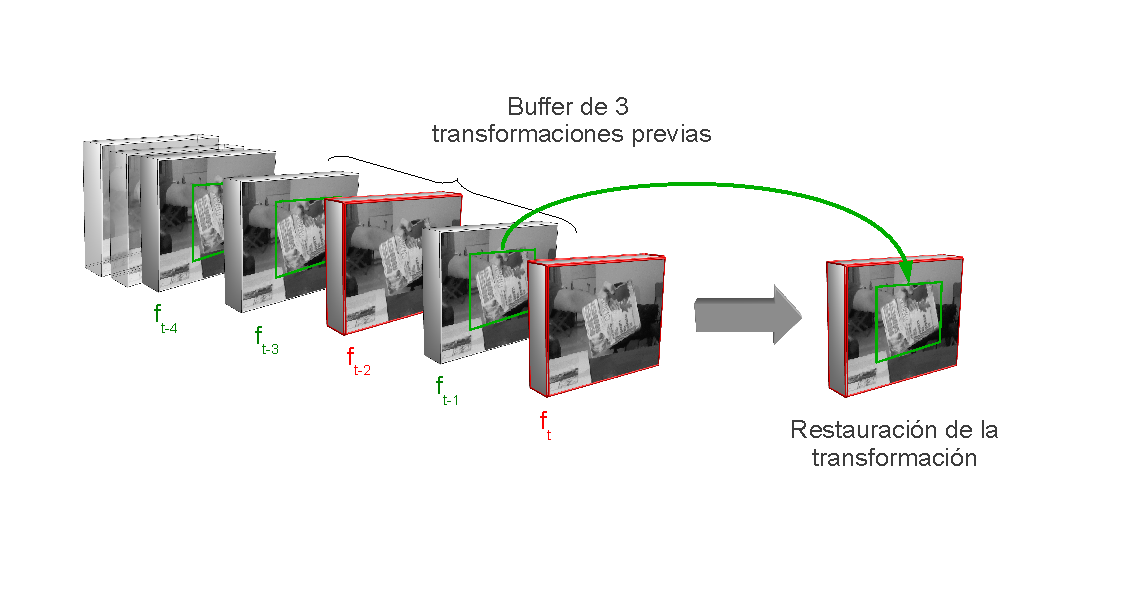
\includegraphics[scale=0.6]{../../figs/restauracion_transfromacion}
       \caption[\small{Esquema de restauración de la última transformación válida}]{\small{Esquema de restauración de la última transformación válida.}}
    \label{fig:restauracion_transformacion} 
  \end{figure}
\end{frame}
\subsection*{}
\begin{frame}{RA en el flujo de video}
  \begin{itemize}
    \item Se utiliza $H^{-1}$ para superponer la imagen virtual en la perspectiva correcta en el flujo de video.
      \note[item]{plane (usually the imager plane) by the following simple eqns: 
      p_dest = H * p_src,  p_src = H^ -1 * p_dest 
      In this case, p_dest is the image plane, p_src is the world plane. To solve for the world pts, use the 2nd equn above}
      \note[item]{H mapea puntos de una primer imagen a puntos en una segunda imagen}
    \item Existe una interpolación debido a la transformación de píxeles.
  \end{itemize}

  \begin{figure}[tbhp]
   \centering
        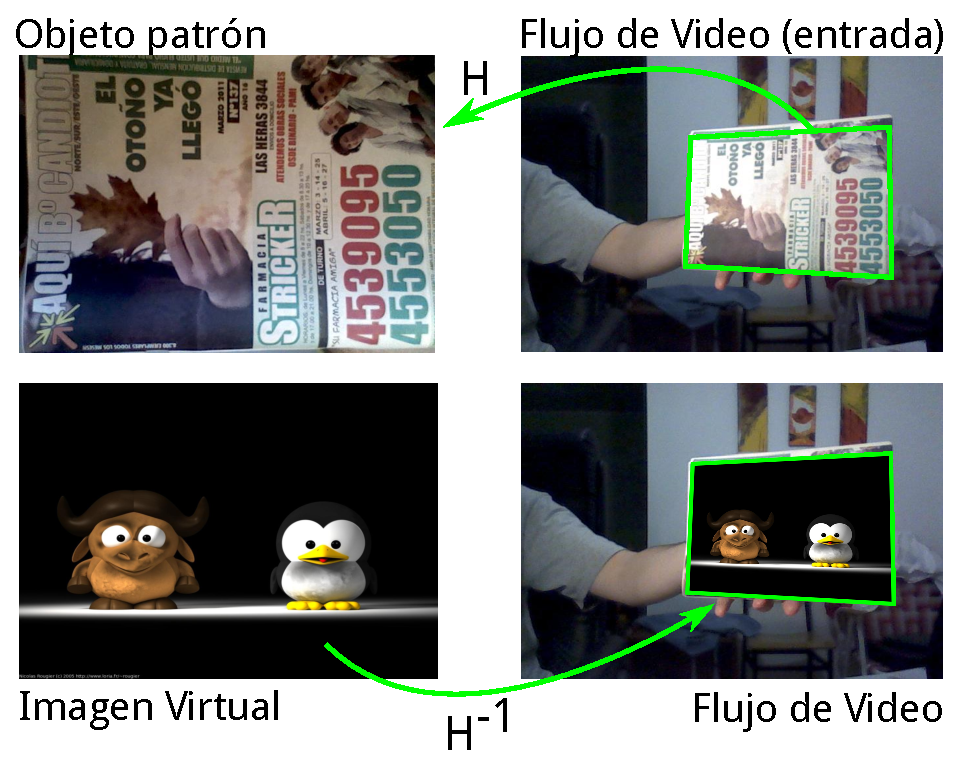
\includegraphics[scale=0.4]{../../figs/transfperspectiva_presentacion}
    \caption[\small{Esquema de transformación perspectiva}]{\small{Esquema de transformación perspectiva utilizando la homografía $H$.}}
   \label{fig:transf_pespectiva}
  \end{figure}
\end{frame}